\documentclass[aspectratio=169]{beamer}
\usetheme[pageofpages=of,% String used between the current page and the
                         % total page count.
          bullet=circle,% Use circles instead of squares for bullets.
          titleline=true,% Show a line below the frame title.
          alternativetitlepage=true,% Use the fancy title page.
	  titlepagelogo=logo-circl.pdf,% Logo for the first page.
%          watermark=watermark-polito,% Watermark used in every page.
%          watermarkheight=100px,% Height of the watermark.
%          watermarkheightmult=4,% The watermark image is 4 times bigger
                                % than watermarkheight.
          ]{Torino}

\usepackage[utf8x]{inputenc}
\usepackage{listings}
\usepackage{soul}
\usepackage{siunitx}
\usepackage{booktabs}
%\lstset{ 
%  backgroundcolor=\color{white},   % choose the background color; you must add \usepackage{color} or \usepackage{xcolor}
%  basicstyle=\footnotesize,        % the size of the fonts that are used for the code
%  breakatwhitespace=false
%}

\usepackage{tikz}
\usetikzlibrary{shapes,snakes,automata,positioning,matrix,fit}


\usepackage[listings]{tcolorbox}
\usepackage{xcolor}
\usepackage{colortbl}
\definecolor{mygreen}{rgb}{0,0.6,0}
\definecolor{mygreen2}{rgb}{0,0.56,0.16}
\definecolor{myred}{rgb}{0.6,0.066,0.066}
\definecolor{redCIRCL}{RGB}{213,43,30}
\definecolor{mygray}{rgb}{0.5,0.5,0.5}
\definecolor{mymauve}{rgb}{0.58,0,0.82}
\definecolor{mygray}{gray}{0.9}
\definecolor{mywhite}{rgb}{1,1,1}
\definecolor{myblack}{rgb}{0,0,0}
\definecolor{mybeige}{HTML}{eeeeee}
%\usepackage{tcolorbox}
\usepackage[listings]{tcolorbox}
\tcbuselibrary{listings}

\lstdefinestyle{code}{ %
  backgroundcolor=\color{mybeige},   % choose the background color; you must add \usepackage{color} or \usepackage{xcolor}; should come as last argument
  basicstyle=\footnotesize\ttfamily,        % the size of the fonts that are used for the code
  breakatwhitespace=false,         % sets if automatic breaks should only happen at whitespace
  breaklines=true,                 % sets automatic line breaking
  captionpos=b,                    % sets the caption-position to bottom
  commentstyle=\color{mygreen},    % comment style
  deletekeywords={...},            % if you want to delete keywords from the given language
  escapeinside={\%*}{*)},          % if you want to add LaTeX within your code
  extendedchars=true,              % lets you use non-ASCII characters; for 8-bits encodings only, does not work with UTF-8
  frame=single,	                   % adds a frame around the code
  keepspaces=true,                 % keeps spaces in text, useful for keeping indentation of code (possibly needs columns=flexible)
  keywordstyle=\color{blue},       % keyword style
  language=Python,                 % the language of the code
  morekeywords={*,...},           % if you want to add more keywords to the set
  numbers=left,                    % where to put the line-numbers; possible values are (none, left, right)
  numbersep=5pt,                   % how far the line-numbers are from the code
  numberstyle=\tiny\color{myblack}, % the style that is used for the line-numbers
  rulecolor=\color{black},         % if not set, the frame-color may be changed on line-breaks within not-black text (e.g. comments (green here))
  showspaces=false,                % show spaces everywhere adding particular underscores; it overrides 'showstringspaces'
  showstringspaces=false,          % underline spaces within strings only
  showtabs=false,                  % show tabs within strings adding particular underscores
  stepnumber=1,                    % the step between two line-numbers. If it's 1, each line will be numbered
  stringstyle=\color{mymauve},     % string literal style
  tabsize=2,	                   % sets default tabsize to 2 spaces
  title=\lstname                   % show the filename of files included with \lstinputlisting; also try caption instead of title
}
\lstdefinestyle{bash}{ %
  backgroundcolor=\color{black!85},   % choose the background color; you must add \usepackage{color} or \usepackage{xcolor}; should come as last argument
  basicstyle=\footnotesize\color{mywhite},        % the size of the fonts that are used for the code
  breakatwhitespace=false,         % sets if automatic breaks should only happen at whitespace
  breaklines=true,                 % sets automatic line breaking
  captionpos=b,                    % sets the caption-position to bottom
  commentstyle=\color{mygreen},    % comment style
  deletekeywords={...},            % if you want to delete keywords from the given language
  escapeinside={\%*}{*)},          % if you want to add LaTeX within your code
  extendedchars=true,              % lets you use non-ASCII characters; for 8-bits encodings only, does not work with UTF-8
  frame=single	                   % adds a frame around the code
  keepspaces=true,                 % keeps spaces in text, useful for keeping indentation of code (possibly needs columns=flexible)
  keywordstyle=\color{white}\bfseries,       % keyword style
  language=bash,                 % the language of the code
  morekeywords={*,$,git, clone,... },           % if you want to add more keywords to the set
  numbers=left,                    % where to put the line-numbers; possible values are (none, left, right)
  numbersep=5pt,                   % how far the line-numbers are from the code
  numberstyle=\tiny\color{mywhite}, % the style that is used for the line-numbers
  rulecolor=\color{black},         % if not set, the frame-color may be changed on line-breaks within not-black text (e.g. comments (green here))
  showspaces=false,                % show spaces everywhere adding particular underscores; it overrides 'showstringspaces'
  showstringspaces=false,          % underline spaces within strings only
  showtabs=false,                  % show tabs within strings adding particular underscores
  stepnumber=1,                    % the step between two line-numbers. If it's 1, each line will be numbered
  stringstyle=\color{mymauve},     % string literal style
  tabsize=2,	                   % sets default tabsize to 2 spaces
  title=\lstname                   % show the filename of files included with \lstinputlisting; also try caption instead of title
}
\lstdefinestyle{default}{ %
  backgroundcolor=\color{white},   % choose the background color; you must add \usepackage{color} or \usepackage{xcolor}; should come as last argument
  basicstyle=\footnotesize\color{black},        % the size of the fonts that are used for the code
  breakatwhitespace=false,         % sets if automatic breaks should only happen at whitespace
  breaklines=true,                 % sets automatic line breaking
  captionpos=b,                    % sets the caption-position to bottom
  commentstyle=\color{mygreen},    % comment style
  deletekeywords={...},            % if you want to delete keywords from the given language
  escapeinside={\%*}{*)},          % if you want to add LaTeX within your code
  extendedchars=true,              % lets you use non-ASCII characters; for 8-bits encodings only, does not work with UTF-8
  frame=single	                   % adds a frame around the code
  keepspaces=true,                 % keeps spaces in text, useful for keeping indentation of code (possibly needs columns=flexible)
  keywordstyle=\color{white}\bfseries,       % keyword style
  language=bash,                 % the language of the code
  morekeywords={*,$,git, clone,... },           % if you want to add more keywords to the set
  numbers=left,                    % where to put the line-numbers; possible values are (none, left, right)
  numbersep=5pt,                   % how far the line-numbers are from the code
  numberstyle=\tiny\color{black}, % the style that is used for the line-numbers
  rulecolor=\color{black},         % if not set, the frame-color may be changed on line-breaks within not-black text (e.g. comments (green here))
  showspaces=false,                % show spaces everywhere adding particular underscores; it overrides 'showstringspaces'
  showstringspaces=false,          % underline spaces within strings only
  showtabs=false,                  % show tabs within strings adding particular underscores
  stepnumber=1,                    % the step between two line-numbers. If it's 1, each line will be numbered
  stringstyle=\color{mymauve},     % string literal style
  tabsize=2,	                   % sets default tabsize to 2 spaces
  title=\lstname                   % show the filename of files included with \lstinputlisting; also try caption instead of title
}
\lstset{style=code}


\AtBeginSection[]{
  \begin{frame}
  \vfill
  \centering
  \begin{beamercolorbox}[sep=8pt,center,shadow=true,rounded=true]{title}
      {\color{white} \usebeamerfont{title}\insertsectionhead}\par%
  \end{beamercolorbox}
  \vfill
  \end{frame}
}

\author{\Large{Alexandre Dulaunoy}\\ \scriptsize{alexandre.dulaunoy@circl.lu}\\ \large{Aurelien Thirion}\\ \scriptsize{aurelien.thirion@circl.lu}\\ %\large{Jean-Louis Huynen}\\ \scriptsize{jean-louis.huynen@circl.lu}\\ \Large{Sami Mokaddem}\\ \scriptsize{sami.mokaddem@circl.lu}
}
\title{AIL Framework for Analysis of Information Leaks}
\subtitle{Practical and Efficient Data-Mining of Suspicious Websites, Forums, Chats and Tor Hidden-Services}
\institute{info@circl.lu}
\date{\today}

\begin{document}


\begin{frame}[t,plain]
\titlepage
\end{frame}


% LINKS
\begin{frame}
\frametitle{Links}
    \begin{itemize}
        \item AIL project website \url{https://ail-project.org}
        \item AIL project open source framework \url{https://github.com/ail-project}
        \item AIL framework \url{https://github.com/ail-project/ail-framework}
        \item Training materials \url{https://github.com/ail-project/ail-training}
	\item Mastodon \url{https://infosec.exchange/@ail_project}
        \item Online chat \url{https://gitter.im/ail-project/community}
    \end{itemize}
    \begin{figure}
        
\includegraphics[scale=0.1, angle=0]{images/ail-project.png}
    \end{figure}
\end{frame}


\section{Legal and Ethics}
\begin{frame}
        \frametitle{Privacy, AIL and GDPR (PII)}
        \begin{itemize}
                \item Many modules in AIL can process personal data and even special categories of data as defined in GDPR (Art. 9).
                \item The data controller is often the operator of the AIL framework (limited to the organisation) and has to define {\bf legal grounds for processing personal data}.
                \item To help users of AIL framework, a document is available which describe points of AIL in regards to the regulation\footnote{\url{https://www.circl.lu/assets/files/information-leaks-analysis-and-gdpr.pdf}}.
        \end{itemize}
\end{frame}

\begin{frame}
        \frametitle{Potential legal grounds}
        \begin{itemize}
                \item {\bf Consent of the data subject} is in many cases not feasible in practice and often impossible or illogical to obtain (Art. 6(1)(a)).
                \item Legal obligation (Art. 6(1)(c)) - This legal ground applies mostly to CSIRTs, in accordance with the powers and responsibilities set out in CSIRTs mandate and with their constituency, as they may have the legal obligation to collect, analyse and share information leaks without having a prior consent of the data subject.
				\item Art. 6(1)(f) - Legitimate interest - Recital 49 explicitly refers to CSIRTs’ right to process personal data provided that they have a legitimate interest but not colliding with fundamental rights and freedoms of data subject.
        \end{itemize}
\end{frame}

\begin{frame}
        \frametitle{Ethics in Information Security and Cybersecurity}
        \begin{itemize}
        \item The materials and tools presented can open a significant numbers of questions regarding ethics;
        \item Our researches and tools are there for education, supporting the public good and improve incident response;
        \item We ask all users and participants to {\bf follow ethical principles and act professionaly}\footnote{\url{https://www.acm.org/code-of-ethics} \url{https://www.first.org/global/sigs/ethics/ethics-first}}.
        \end{itemize}
\end{frame}

\section{Introduction}
\begin{frame}
        \frametitle{Concepts - Deep Web}
        \begin{itemize}
                \item {\bf Deep Web} is the part of World Wide Web not indexed or directly accessible by standard web search-engines;
                \item This can be content hidden from {\bf crawlers} by requiring a specific access and this can includes private social media, password-protected forums or content protected
                        by different measures such as paywalls or specific security interface to access the information;
                \item A large portion of content accessible via Internet is part of the deep web\footnote{also called invisible web, hidden web or non-indexed web}.
        \end{itemize}
\end{frame}

\begin{frame}
        \frametitle{Concepts - darknet}
        \begin{itemize}
                \item {\bf Darknet} is an overlay network running on top of Internet requiring specific software to access the network and its services;
                \item Tor, I2P and Freenet are the most commonly used ones. Many are used for hidden services access and some for proxy access to the Internet;
		\item There are {\bf legitimate use-cases} for such network but also many {\bf illegal or criminal usage}.
        \end{itemize}
\end{frame}

\begin{frame}
	\frametitle{Lifecycle of collection and analysis}
	\center
\tikzstyle{startstop} = [rectangle, rounded corners, minimum width=3cm, minimum height=0.8cm,text centered, draw=black, fill=red!30]
\tikzstyle{io} = [trapezium, trapezium left angle=70, trapezium right angle=110, minimum width=3cm, minimum height=1cm, text centered, draw=black, fill=blue!30]
\tikzstyle{arrow} = [thick,->,>=stealth]
	\begin{tikzpicture}[node distance=1.4cm]

\node (start) [startstop] {Planning};
\node (collect) [startstop, below of =start] {Collect};
\node (processing) [startstop, below of =collect] {Processing};
\node (analysing) [startstop, below of=processing] {Analysing};
\node (dissemination) [startstop, below of=analysing] {Dissemination};
\draw [arrow] (start) -- (collect);
\draw [arrow] (collect) -- (processing);
\draw [arrow] (processing) -- (analysing);
\draw [arrow] (analysing) -- (dissemination);
%\draw [arrow] (analysing) |- (collect);
\end{tikzpicture}

\end{frame}

\begin{frame}
        \frametitle{Collecting, processing and analysing content - web pages}
        \begin{itemize}
		\item Building a search engine on the web is a challenging task because:
        	\begin{itemize}
			\item it has to crawl webpages,
			\item it has to to make sense of {\bf unstructured data},
			\item it has to {\bf index} these data,
			\item it has to provide a way to retrieve data and structure data (e.g. correlation).
        	\end{itemize}
		\item Doing so on Tor is even more challenging because:

        	\begin{itemize}
			\item services don't always want to be found,
			\item parts of the dataset have to be discarded.
        	\end{itemize}
	\item in each case, it requires a lot of bandwidth, storage and computing power.
        \end{itemize}
\end{frame}


\begin{frame}
        \frametitle{Collecting, processing and analysing content - structured data}
        \begin{itemize}
		\item Some data are structured and are easy to process:
        	\begin{itemize}
			\item metadata!
			\item API responses.
        	\end{itemize}
		\item Some even provide cryptographic evidences:
			        \begin{itemize}

         \item authentication mechanisms between peers,
         \item OpenGPG can leak a lot of metadata
        \begin{itemize}
          \item key ids,
          \item subject of email in thunderbird,
        \end{itemize}
          \item Bitcoin's Blockchain is public,
          \item pivoting on these data with external sources yields interesting results.
        \end{itemize}


        \end{itemize}
\end{frame}

\section{AIL design Objectives}
\begin{frame}
\frametitle{Objectives of the session}
    \begin{itemize}
        \item Show how to use and extend an open source tool to monitor web pages, pastes, chats, forums and hidden services
        \item Explain challenges and the design of the AIL open source framework
        \item Review different {\bf collection mechanisms} and {\bf sources}
        \item Learn how to create new modules
        \item Learn how to use, install and start AIL
        \item {\bf Supporting investigation using the AIL framework} and including it in cyber threat intelligence life cycle
    \end{itemize}
\end{frame}

\section{AIL Framework}
\begin{frame}
    \frametitle{From a requirement to a solution: AIL Framework}
    \large{History:}
    \begin{itemize}
        \item AIL initially started as an \textbf{internship project} (2014) to evaluate the feasibility to automate the analysis of (un)structured information to find leaks.
        \item In 2019, AIL framework is an \textbf{open source software} in Python. The software is actively used (and maintained) by CIRCL and many organisations.
        \item In 2020, AIL framework is now a complete project called \textbf{ail project}\footnote{\url{https://github.com/ail-project/}}.
        \item In 2023, AIL framework version 5.0 released with new datastorage back-end.
    \end{itemize}
\end{frame}

\section{Capabilities Overview}

\begin{frame}
    \frametitle{Common usage}
        \begin{itemize}
                \item {\bf Check} if mail/password/other sensitive information (terms tracked) leaked
                \item {\bf Detect} reconnaissance of your infrastructure
                \item {\bf Search} for leaks inside an archive
                \item {\bf Monitor} and crawl chats/websites
        \end{itemize}
\end{frame}

\begin{frame}
    \frametitle{Support CERT and Law Enforcement activities}
        \begin{itemize}
            \item Proactive investigation: leaks detection
            \begin{itemize}
		        \item List of emails and passwords
		        \item Leaked database
		        \item AWS Keys
		        \item Credit-cards
		        \item PGP private keys
		        \item Certificate private keys
		    \end{itemize}
		    \item Feed Passive DNS or any passive collection system
		    \item CVE and PoC of vulnerabilities most used by attackers
		\end{itemize}
\end{frame}

\begin{frame}
    \frametitle{Support CERT and Law Enforcement activities}
    	\begin{itemize}
		    \item Website monitoring
		    	\begin{itemize}
				    \item monitor booters
				    \item Detect encoded exploits (WebShell, malware encoded in Base64, ...)
				    \item SQL injections
		    	\end{itemize}
		    \item Chat/Channel monitoring
		        \begin{itemize}
				    \item Monitor Threat Actor Chat and Community Activities
		        \end{itemize}
		    \item Automatic and manual submission to threat sharing and incident response platforms
			    \begin{itemize}
				    \item MISP
				    \item \textit{flowIntel (Coming soon)}
			    \end{itemize}
		    \item Term/Regex/YARA monitoring for local companies/government
		    \item YARA Retro Hunt
        \end{itemize}
\end{frame}

\section{Sources of leaks}

\begin{frame}
    \frametitle{Mistakes from users:}
        \begin{figure}
            \includegraphics[scale=0.4]{images/git-pass.png}
        \end{figure}
\end{frame}

\begin{frame}
    \frametitle{Sources of Leaks: Paste Monitoring}
    \begin{itemize}
        \item \textbf{Example:} \url{https://gist.github.com/}
        \begin{itemize}
            \item Easily stores and shares text online
            \item Used by programmers and legitimate users
            \item[] $\rightarrow$ Source code \& configuration information
        \end{itemize}
        \vspace{0.3cm}
        \item \textbf{Abused by attackers to store:}
        \begin{itemize}
            \item Lists of vulnerable/compromised sites
            \item Software vulnerabilities (e.g., exploits)
            \item Database dumps
            \item[] $\rightarrow$ User data
            \item[] $\rightarrow$ Credentials
            \item[] $\rightarrow$ Credit card details
            \item Increasingly more sensitive information
        \end{itemize}
    \end{itemize}
\end{frame}

\begin{frame}[t,plain]
        \frametitle{Examples of pastes (items)}
    \begin{figure}
        \includegraphics[scale=0.32, angle=0]{images/pastes-ex.png}
    \end{figure}
\end{frame}

\begin{frame}
    \frametitle{Why So Many Leaks?}
    \begin{itemize}
        \item \textbf{Economic Interests:} 
        \begin{itemize}
            \item Adversaries promoting services
        \end{itemize}
        \item \textbf{Ransom Model:} 
        \begin{itemize}
            \item To publicly pressure the victims
        \end{itemize}
        \item \textbf{Political Motives:} 
        \begin{itemize}
            \item Adversaries showing off
        \end{itemize}
        \item \textbf{Collaboration:} 
        \begin{itemize}
            \item Criminals need to collaborate
        \end{itemize}
        \item \textbf{Operational Infrastructure:} 
        \begin{itemize}
            \item Malware exfiltrating information on a paste website
        \end{itemize}
        \item \textbf{Mistakes and Errors from Users}
    \end{itemize}
\end{frame}

\begin{frame}
    \frametitle{What's your role while discovering such leak?}
    \begin{center}
        \large{As a CSIRT, we must address this issue.}
    \end{center}
    \vspace{0.5cm}

    \begin{itemize}
        \item \textbf{Contacting companies or organizations} responsible for accidental leaks
        \item \textbf{Engaging with the media} about specific leak cases to ensure practical and factual reporting
        \item \textbf{Evaluating the economic landscape} for cyber criminals (e.g., DDoS booters\footnote{\url{https://github.com/D4-project/}} or the resale of personal information - comparing reality versus media coverage)
        \item \textbf{Analyzing collateral effects} of malware, software vulnerabilities, or data exfiltration
    \end{itemize}

\end{frame}
%\begin{frame}
%    \frametitle{Paste monitoring at CIRCL: Statistics}
%    \begin{itemize}
%        \item Monitored paste sites: 27
%            \begin{itemize}
%               \item \textit{gist.github.com}
%               \item \textit{ideone.com}
%                \item \textit{...}
%            \end{itemize}
%   \end{itemize}
%    \begin{table}[h]
%		\centering
%		\begin{tabular}{|lrrr|}
%		    \hline
%		    \rowcolor{lightgray} & 2016 & 2017 & 08.2018\\
%		    Collected pastes & 18,565,124 & 19,145,300 & 11,591,987 \\
%		    Incidents & 244 & 266 & 208\\
%		    \hline
%		\end{tabular}
%		\caption{Pastes collected and incident\footnote{\url{http://www.circl.lu/pub/tr-46}} raised by CIRCL}
%		\label{circlStats}
%	\end{table}
%\end{frame}





\section{Current capabilities}

\begin{frame}
    \frametitle{High Level Overview}
    \begin{center}
        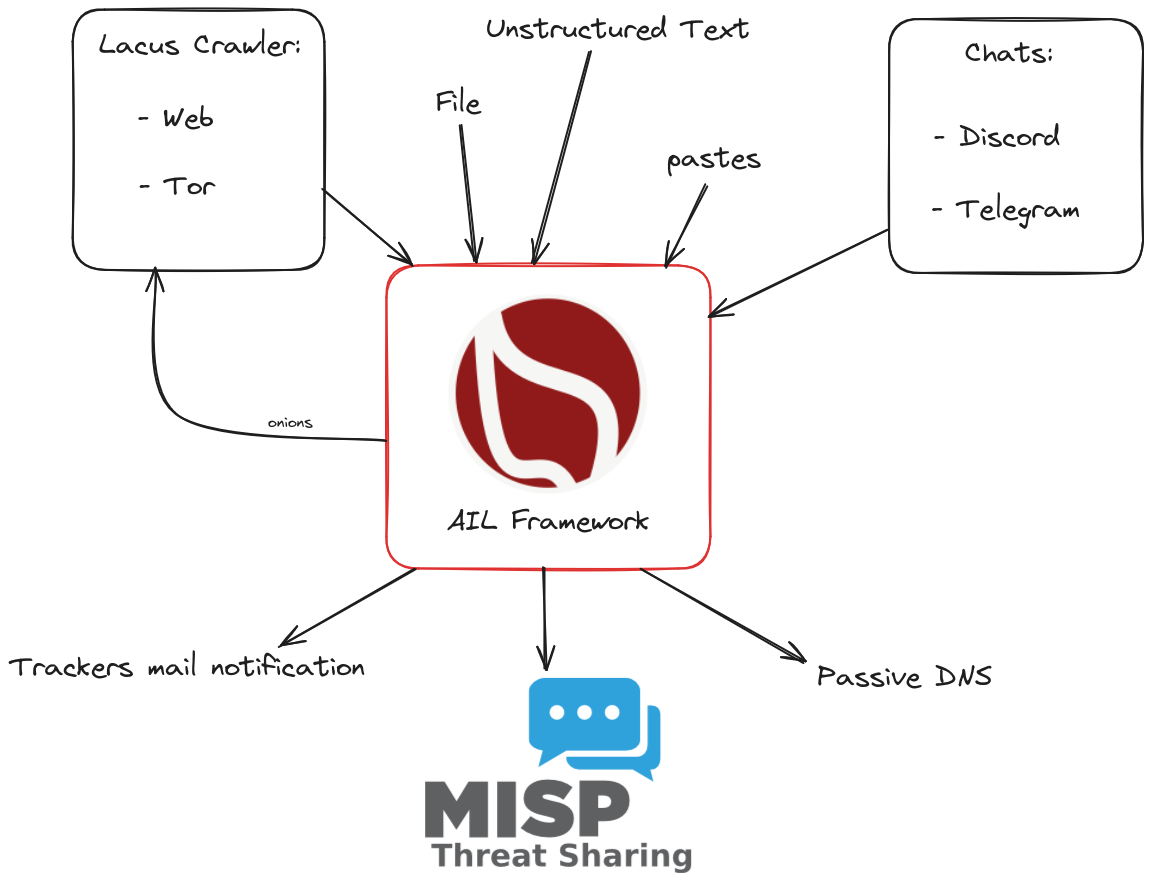
\includegraphics[scale=0.22]{images/ail-overview.png}
    \end{center}
\end{frame}


\begin{frame}
    \frametitle{AIL Framework: Extensible capabilities}
    \begin{itemize}
        \item Extending AIL to add a new {\bf analysis module} can be done in 50 lines of Python
        \item The framework {\bf supports multi-processors/cores by default}. Any analysis module can be started multiple times to support faster processing during peak times or bulk import
        \item \textbf{Multiple} concurrent \textbf{data inputs}
        \item Tor Crawler (handle cookies authentication)
        \item Feeders: Discord, Telegram, ...
    \end{itemize}
\end{frame}

\begin{frame}
    \frametitle{Analysis of unstructured information}
    \begin{center}
        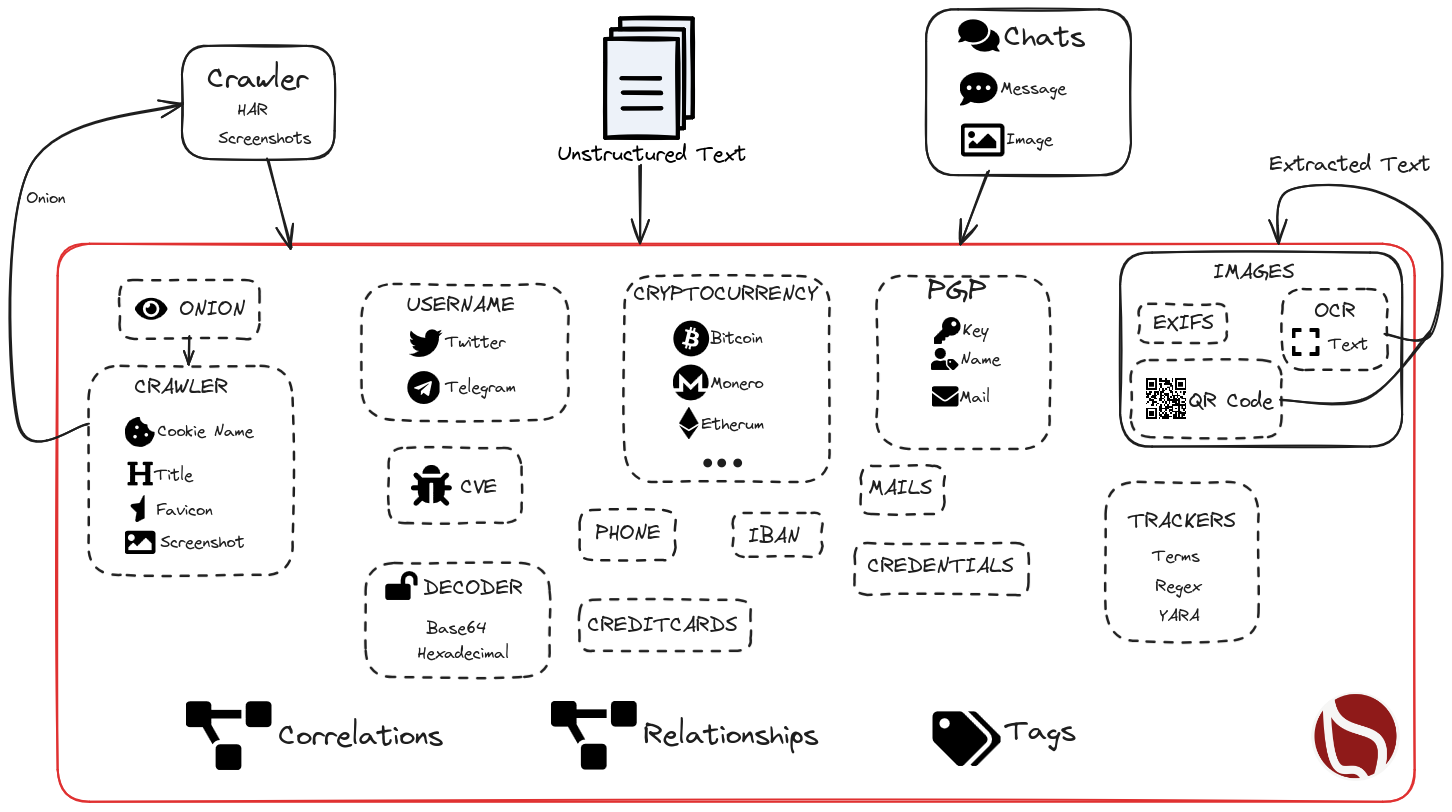
\includegraphics[scale=0.225]{images/ail-internal.png}
    \end{center}
\end{frame}

\begin{frame}
    \frametitle{AIL Framework: Features}
    \begin{itemize}
        \item Extracting \textbf{credit card numbers, credentials, phone numbers, ...}
        \item Extracting and validating potential \textbf{hostnames}
        \item Keeps track of \textbf{duplicates}
        \item Submission to threat sharing and incident response platforms (\textbf{MISP}) % and \textbf{flowIntel})
        \item \textbf{Full-text indexer} to index unstructured information
        \item \textbf{Tagging} for classification and searches
        \item Terms, sets, regex and YARA \textbf{tracking, occurrences, and history}
        \item Archives, files, and raw \textbf{submission} from the UI
        \item Correlation engine based on PGP ID, cryptocurrencies, decoded (Base64, ...), usernames, cookie names, and many selectors to find relationships
        \item And many more
    \end{itemize}
\end{frame}


\begin{frame}
    \frametitle{Trackers - Retro Hunt}
        \begin{itemize}
        	\item Search and monitor specific keywords/patterns
        	\begin{itemize}
            	\item Automatic Tagging
            	\item Email Notifications
            \end{itemize}
            \item Track Word
            \begin{itemize}
            	\item ddos
            \end{itemize}
            \item Track Set
            \begin{itemize}
            	\item booter,ddos,stresser;2
            \end{itemize}
            \item Track Regex
            \begin{itemize}
            	\item circl\textbackslash.lu
            \end{itemize}
            \item YARA rules
            	\begin{itemize}
            	\item https://github.com/ail-project/ail-yara-rules
            \end{itemize}
        \end{itemize}
\end{frame}

\begin{frame}
    \frametitle{YARA Tracker}
        \begin{figure}
            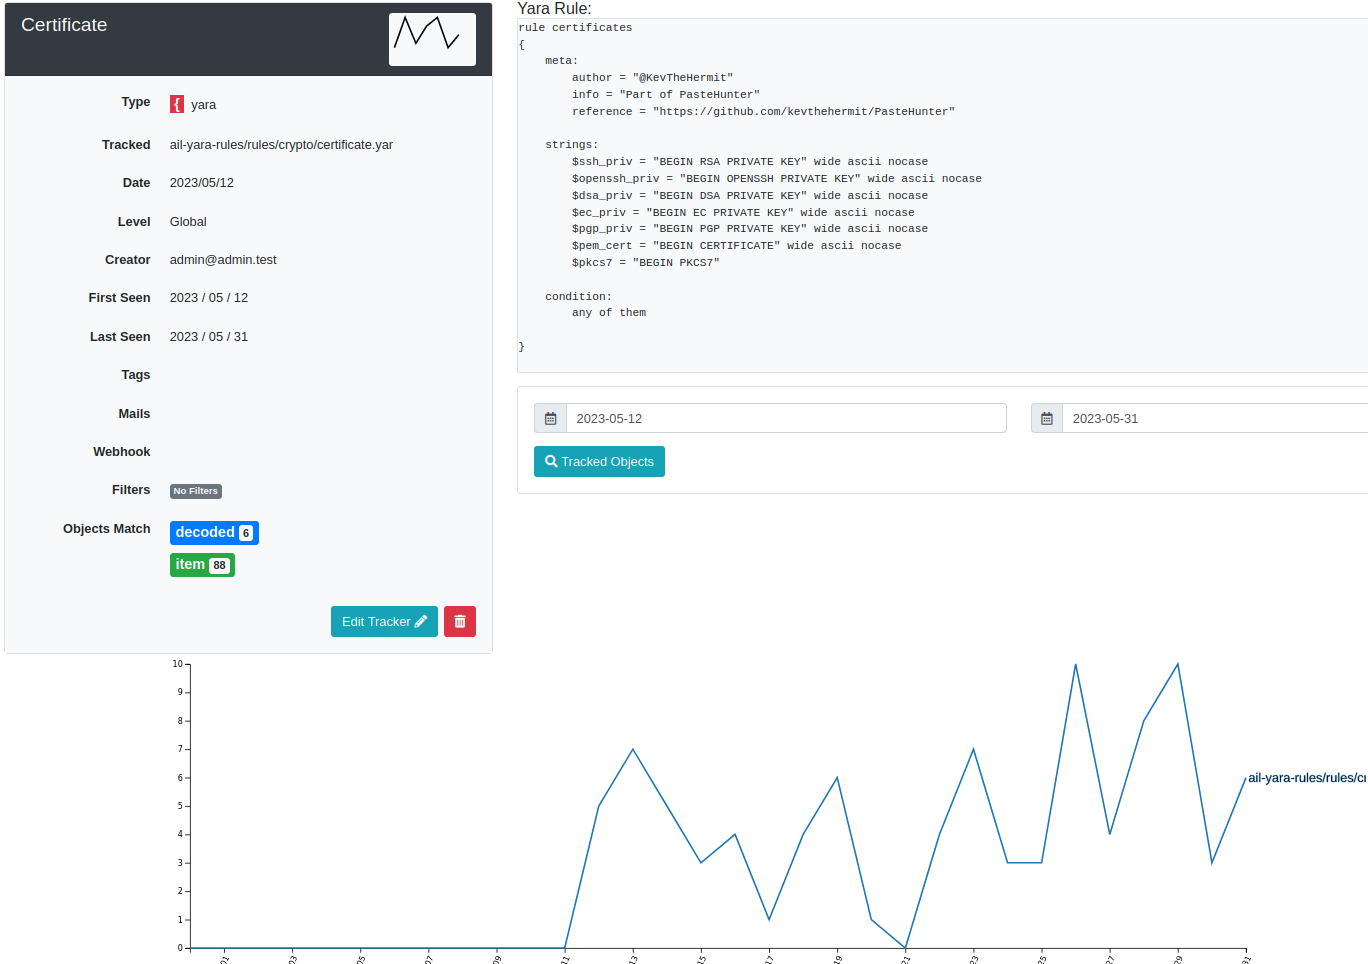
\includegraphics[scale=0.22]{screenshot/tracker_yara.png}
        \end{figure}
\end{frame}

\begin{frame}
    \frametitle{Trackers - Practical part}
        \begin{itemize}
        	\item \textbf{Create and test} your own tracker
        	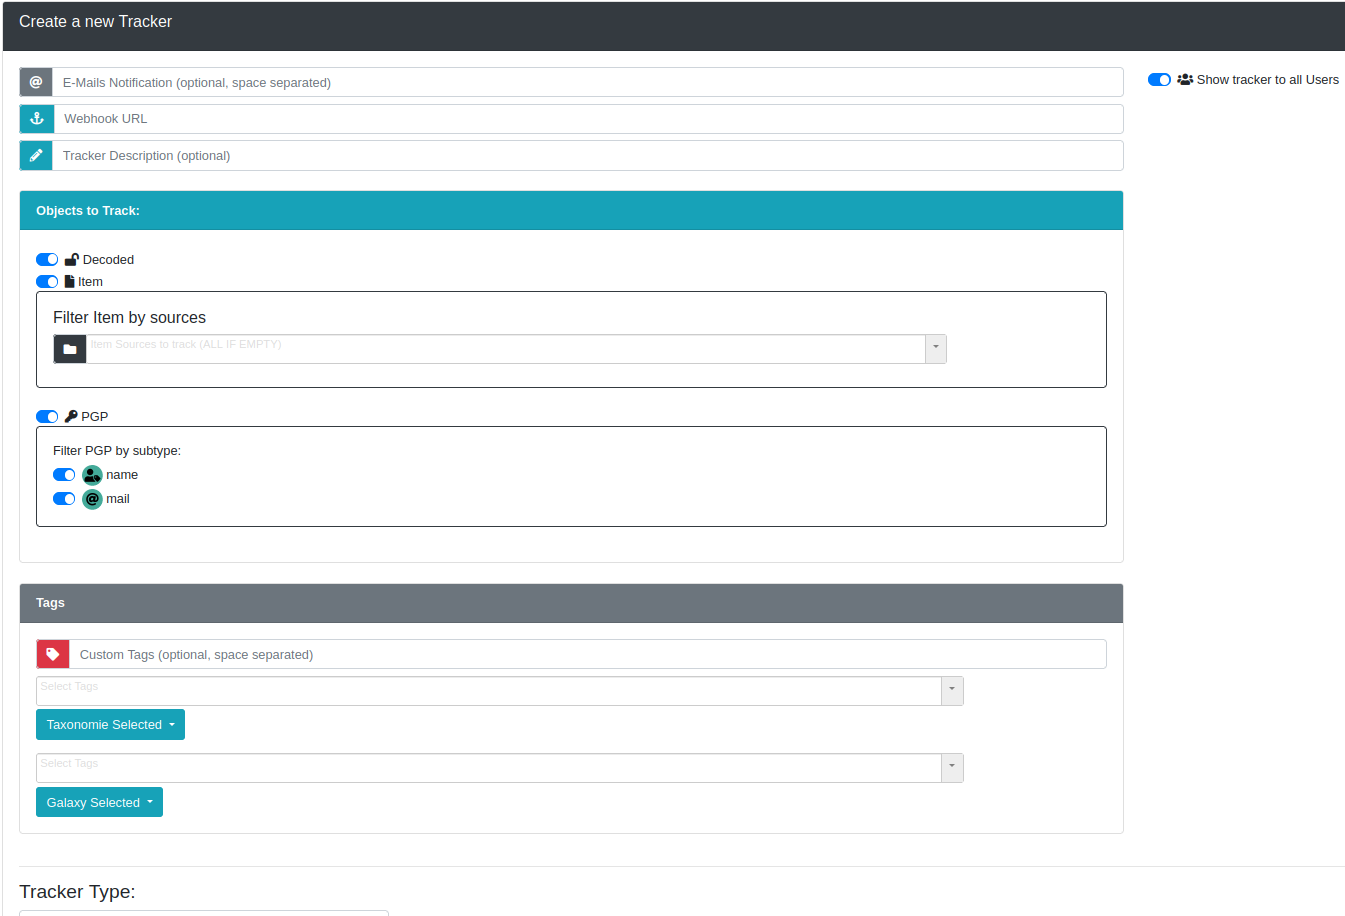
\includegraphics[scale=0.21]{screenshot/tracker_create.png}
        \end{itemize}
\end{frame}

\begin{frame}
    \frametitle{Retro Hunt}
        \begin{figure}
            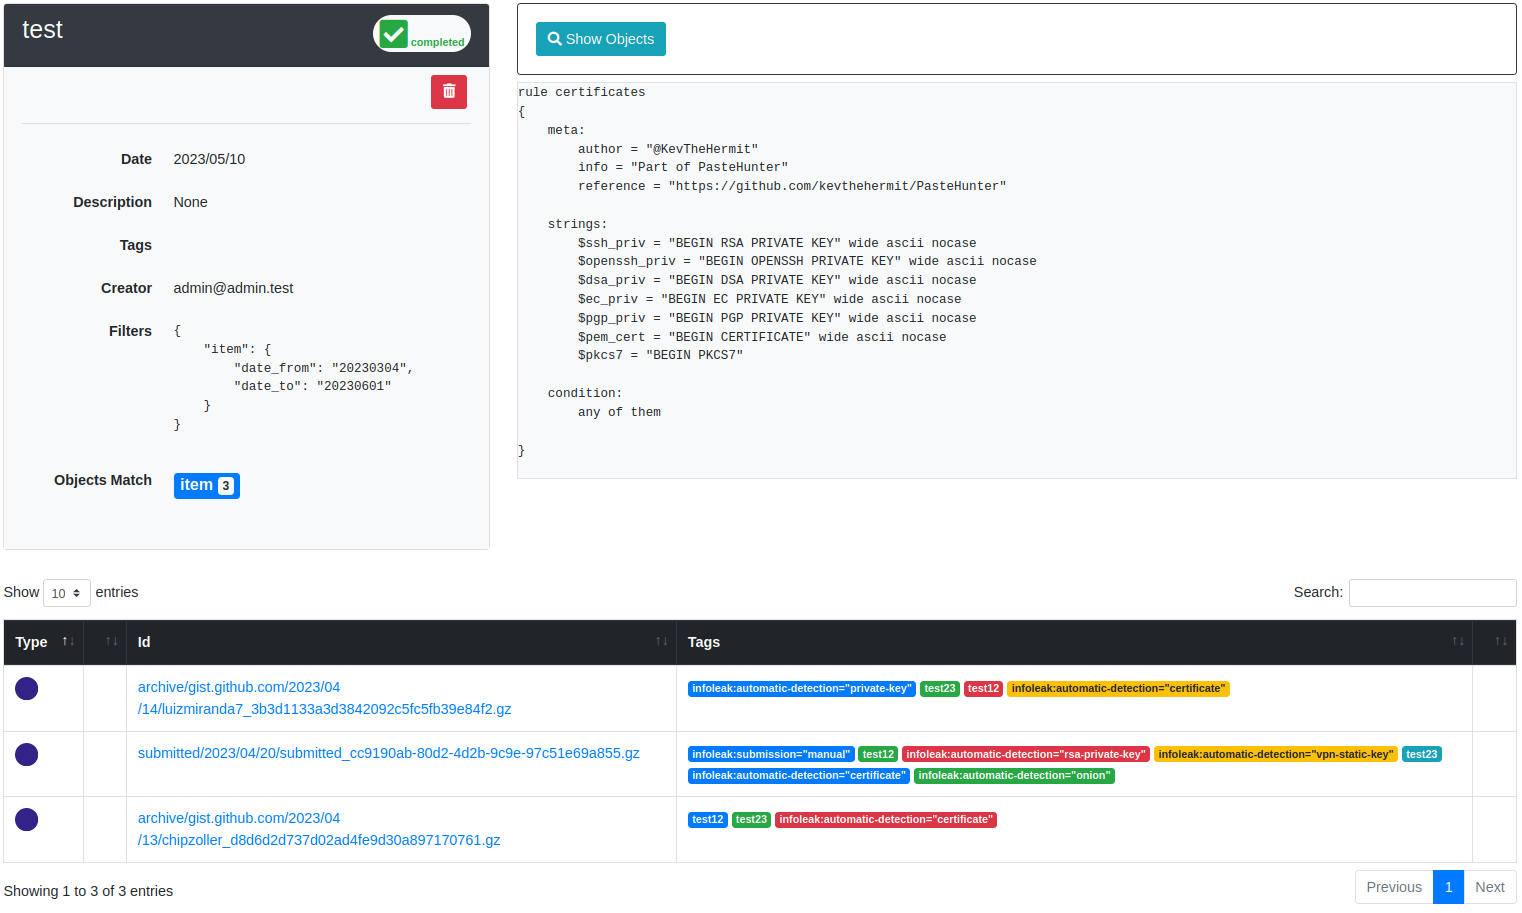
\includegraphics[scale=0.22]{screenshot/retro_hunt.png}
        \end{figure}
\end{frame}

\begin{frame}
    \frametitle{Recon and intelligence gathering tools}
        \begin{itemize}
            \item {\bf Attacker also share informations}
            \item Recon tools detected: 94
            \begin{itemize}
            	\item sqlmap
            	\item dnscan
            	\item whois
            	\item msfconsole (metasploit)
            	\item dnmap
            	\item nmap
            	\item ...
            \end{itemize}
        \end{itemize}
\end{frame}


\begin{frame}
    \frametitle{Recon and intelligence gathering tools}
        \begin{figure}
            \includegraphics[scale=0.4]{images/recon-paste.png}
        \end{figure}
\end{frame}

% TODO AIL OBJECTS SLIDES

\begin{frame}
    \frametitle{Decoder}
    \begin{itemize}
    	\item Search for encoded strings
    		\begin{itemize}
				\item Base64
				\item Hexadecimal
				\item Binary
			\end{itemize}
    	\item Guess Mime-type
    	\item Items/Domains Correlation
    \end{itemize}
\end{frame}

% \begin{frame}
%     \frametitle{AIL objects}
%     \begin{center}
%         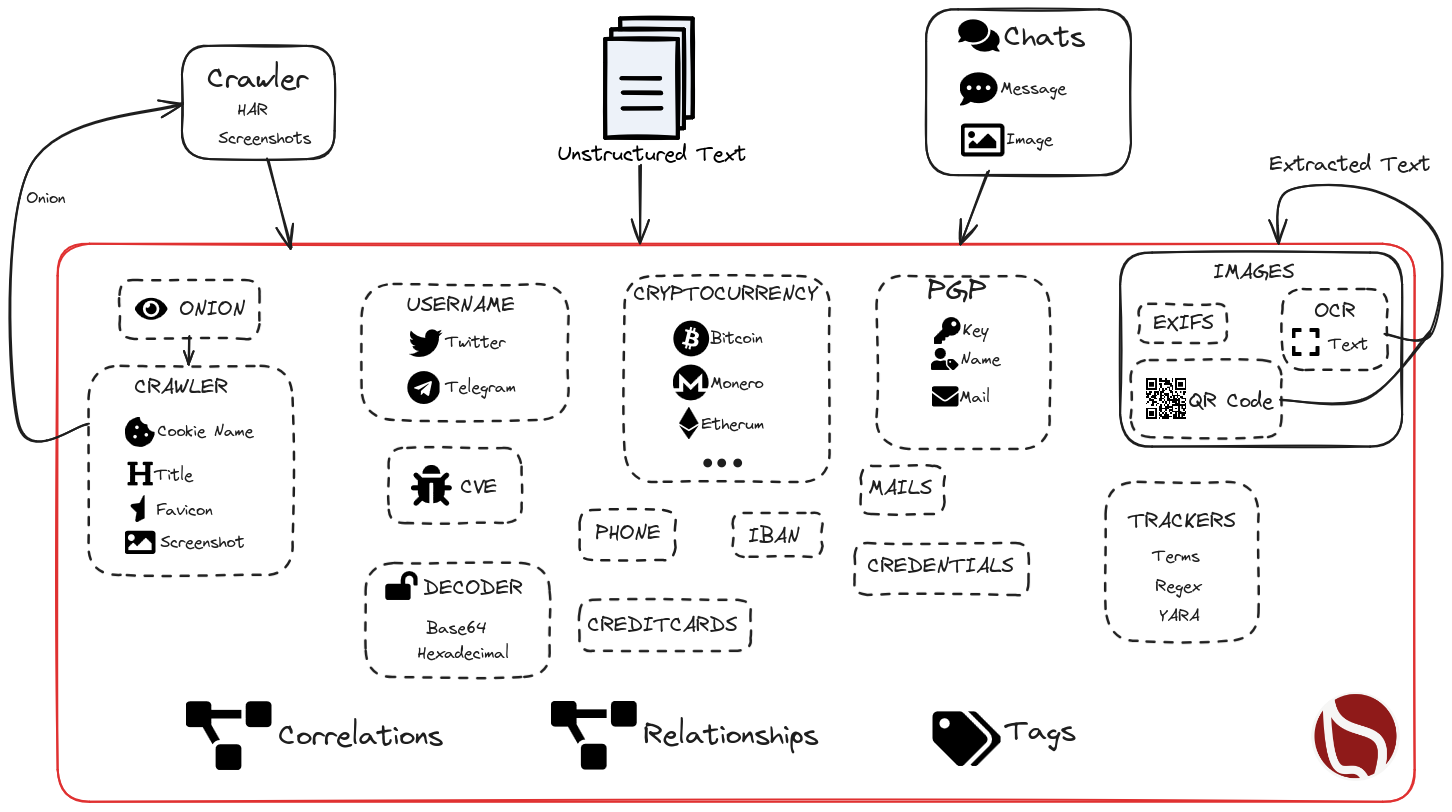
\includegraphics[scale=0.225]{images/ail-internal.png}
%     \end{center}
% \end{frame}

\begin{frame}
    \frametitle{Decoder:}
    \centerline{
        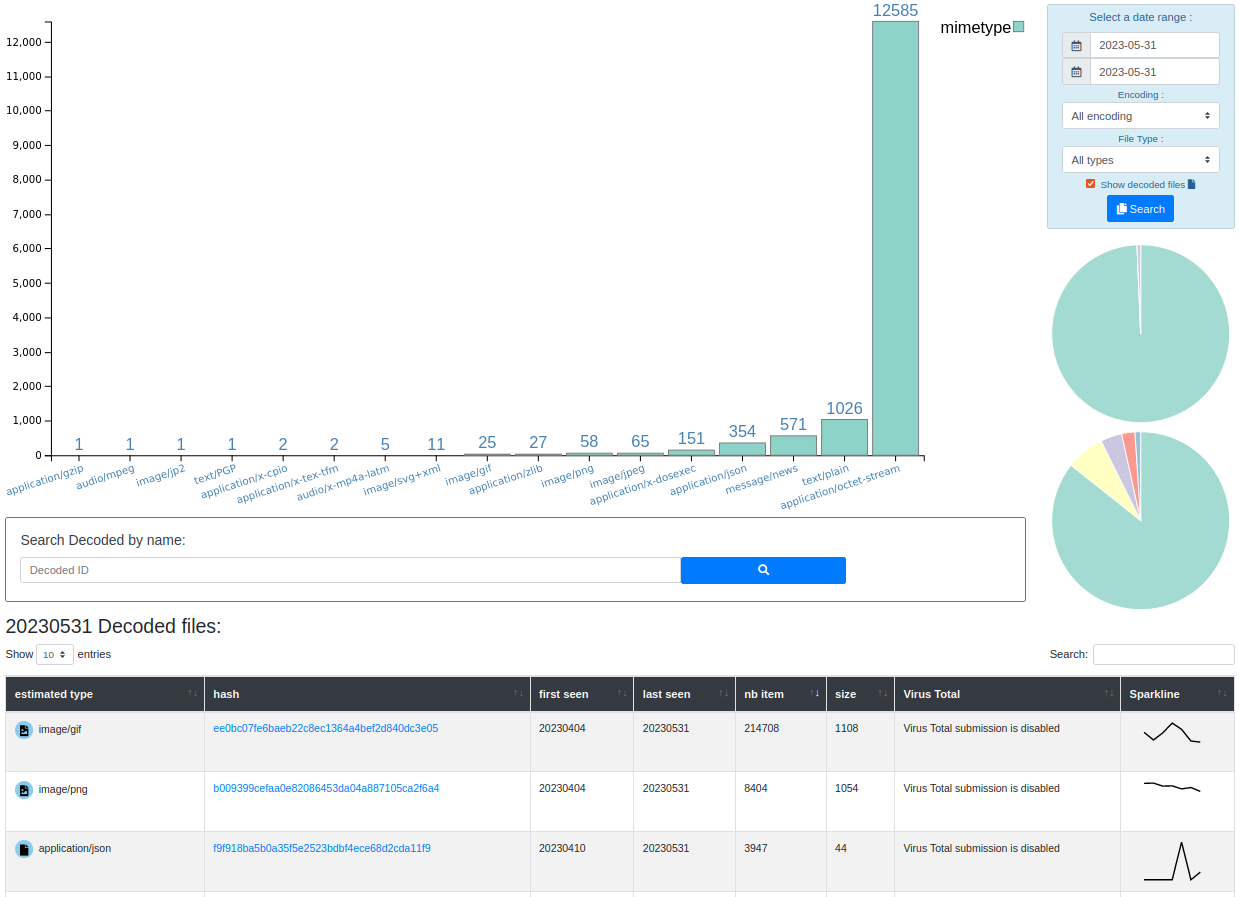
\includegraphics[scale=0.23]{screenshot/decodeds_dashboard.png}
    }
\end{frame}

\begin{frame}
    \frametitle{Decoder:}
    \centerline{
        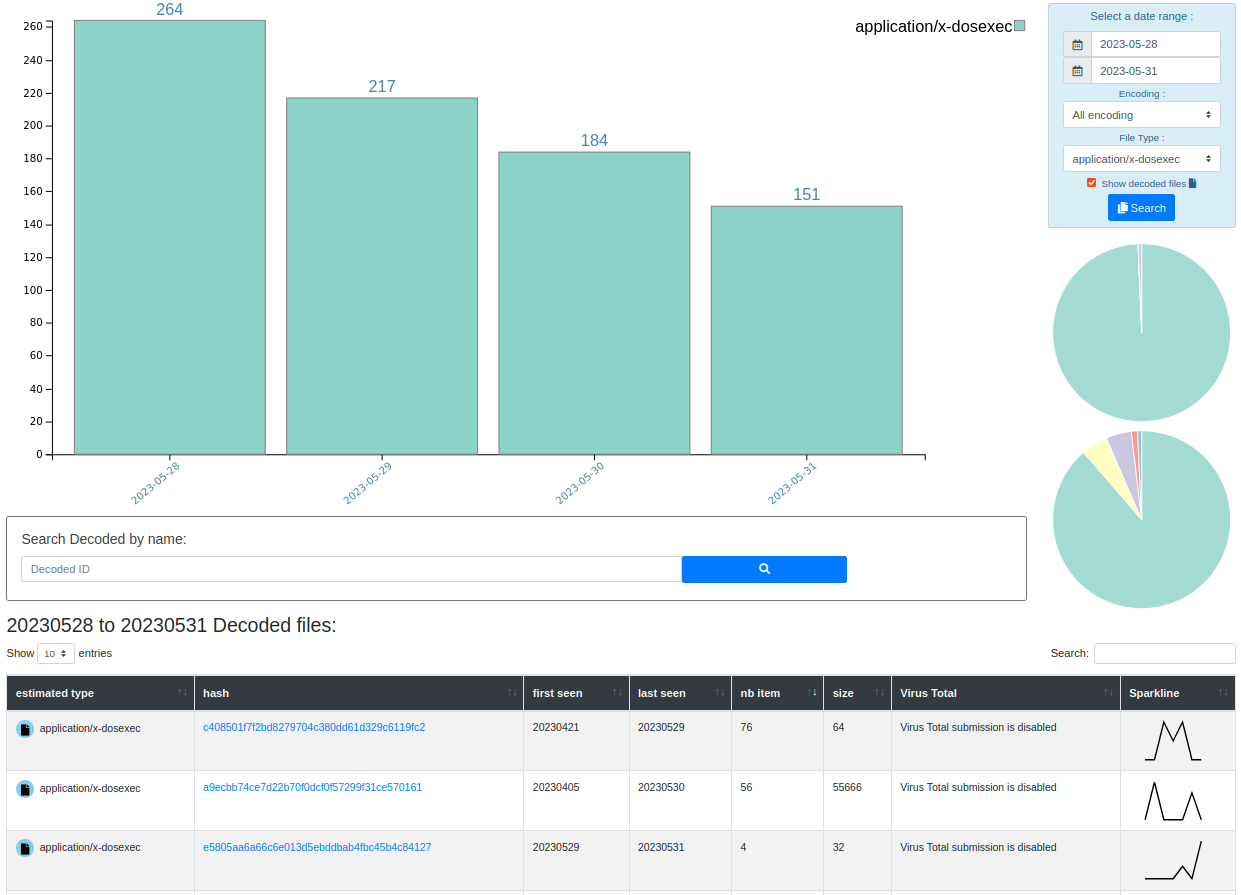
\includegraphics[scale=0.23]{screenshot/decodeds_dos.png}
    }
\end{frame}

\begin{frame}[fragile]{OCR: Optical Character Recognition}
    \begin{columns}[T,onlytextwidth]
        \column{0.45\textwidth}
            \centering
            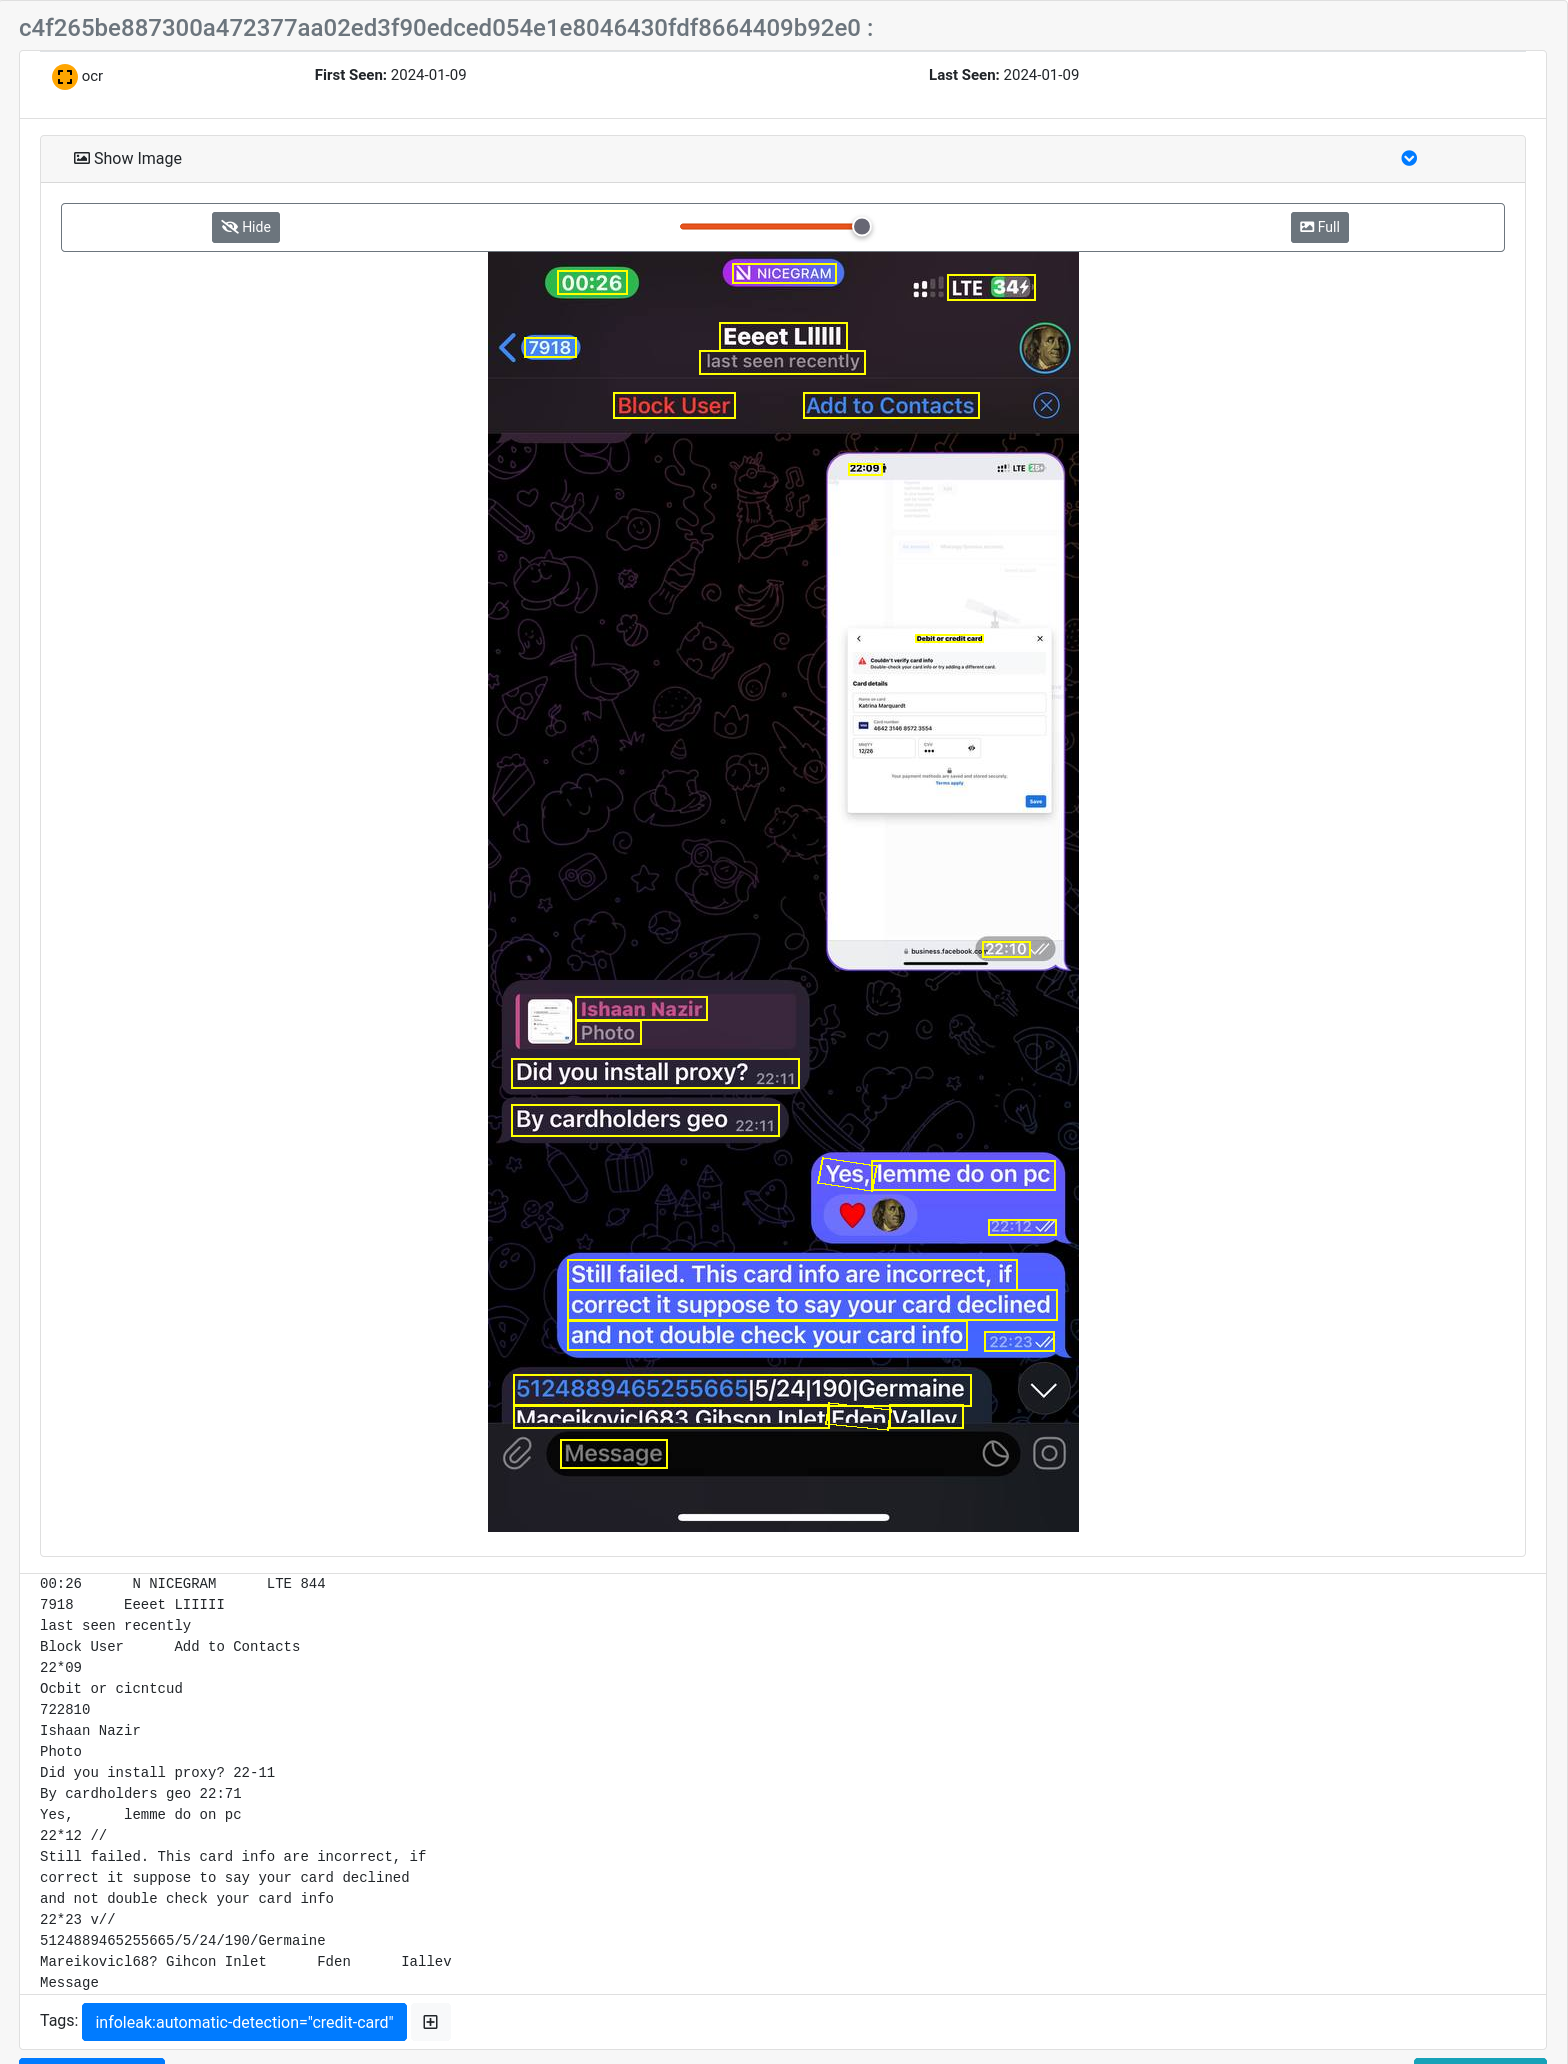
\includegraphics[width=\linewidth]{screenshot/ocr-1.png}
        \column{0.55\textwidth}
            \begin{itemize}
                \item Threat actors are often verbose and frequently {\bf share extensive details in private channels}.
                \item Many messages contain screenshots and images.
                \item Text detection and extraction are performed across 80+ languages using a CRNN (Convolutional Recurrent Neural Network).
                \item {\bf Enables keyword-based matching and detection}.
            \end{itemize}
    \end{columns}
\end{frame}

\begin{frame}
    \frametitle{QR Code Extractor}
    \begin{center}
        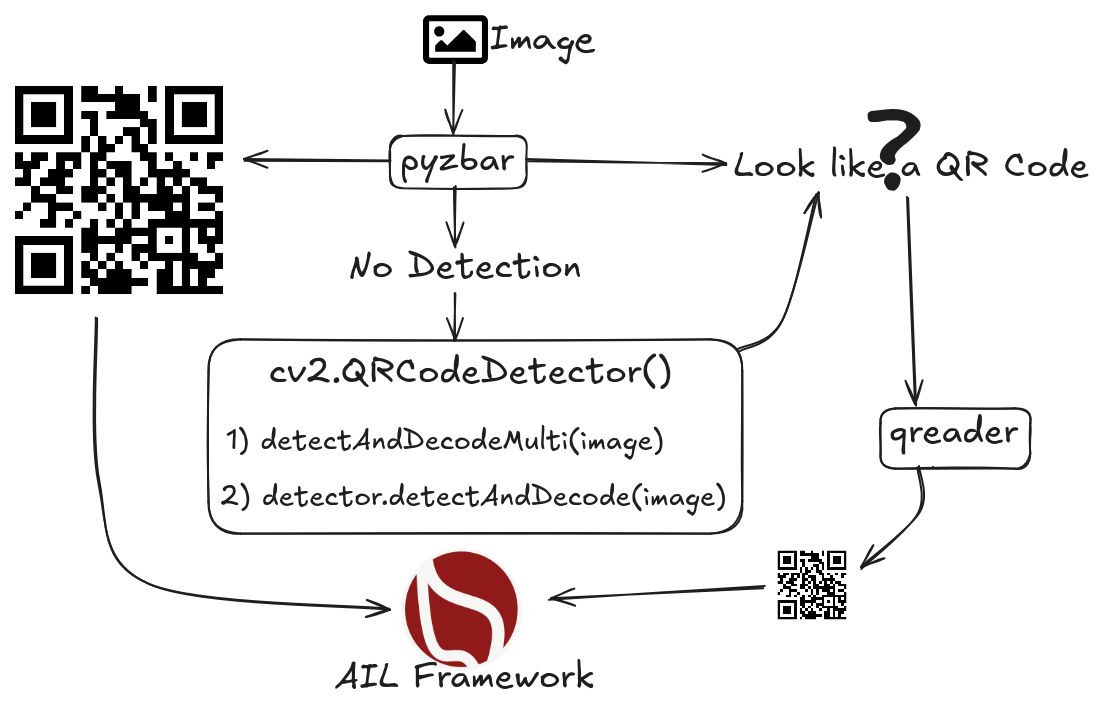
\includegraphics[scale=0.27]{images/qr_decoder.png}
    \end{center}
\end{frame}

\begin{frame}[fragile]{QR Codes}
    \begin{center}
        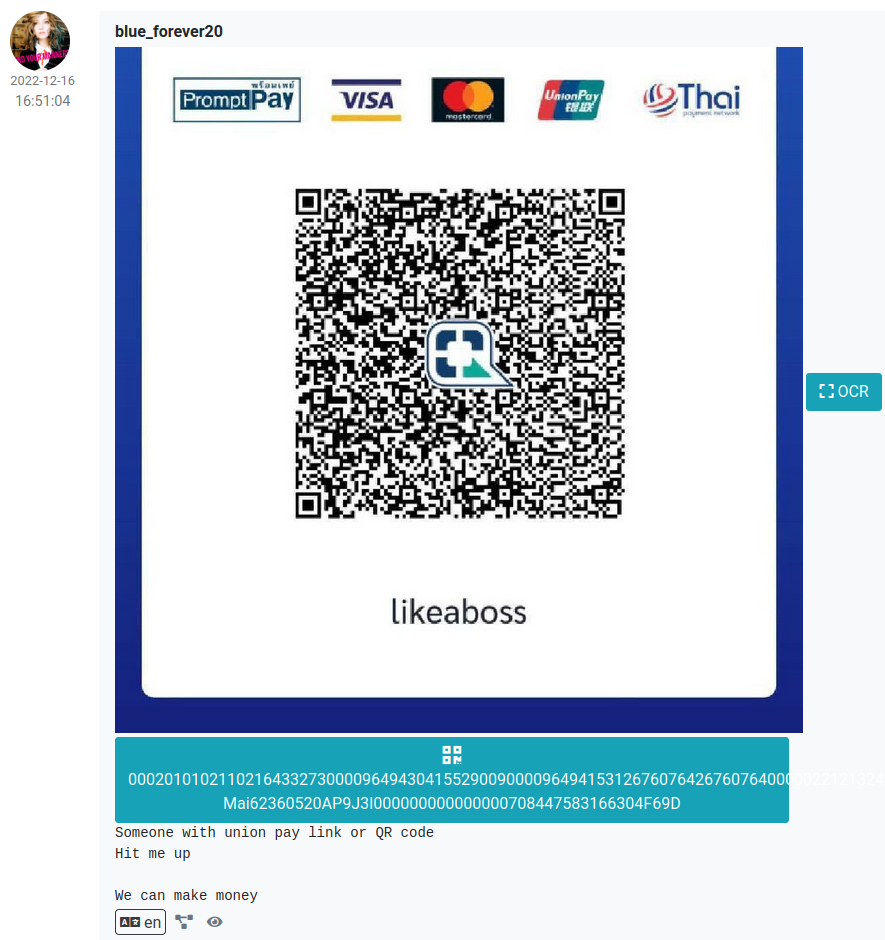
\includegraphics[scale=0.235]{screenshot/qr-pay.png}
    \end{center}
\end{frame}

\begin{frame}[fragile]{Bar Codes}
    \begin{center}
        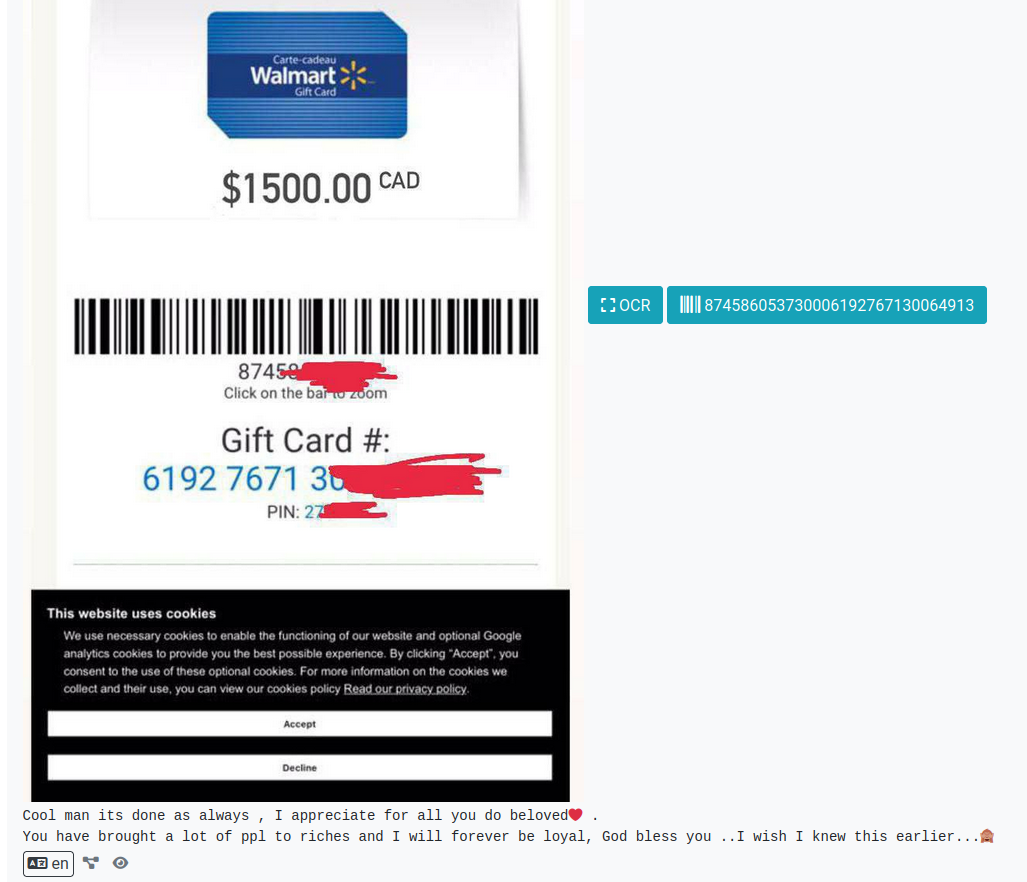
\includegraphics[scale=0.22]{screenshot/barcode.png}
    \end{center}
\end{frame}

\begin{frame}
    \frametitle{Collection - Lacus Crawler}
    \centerline{
        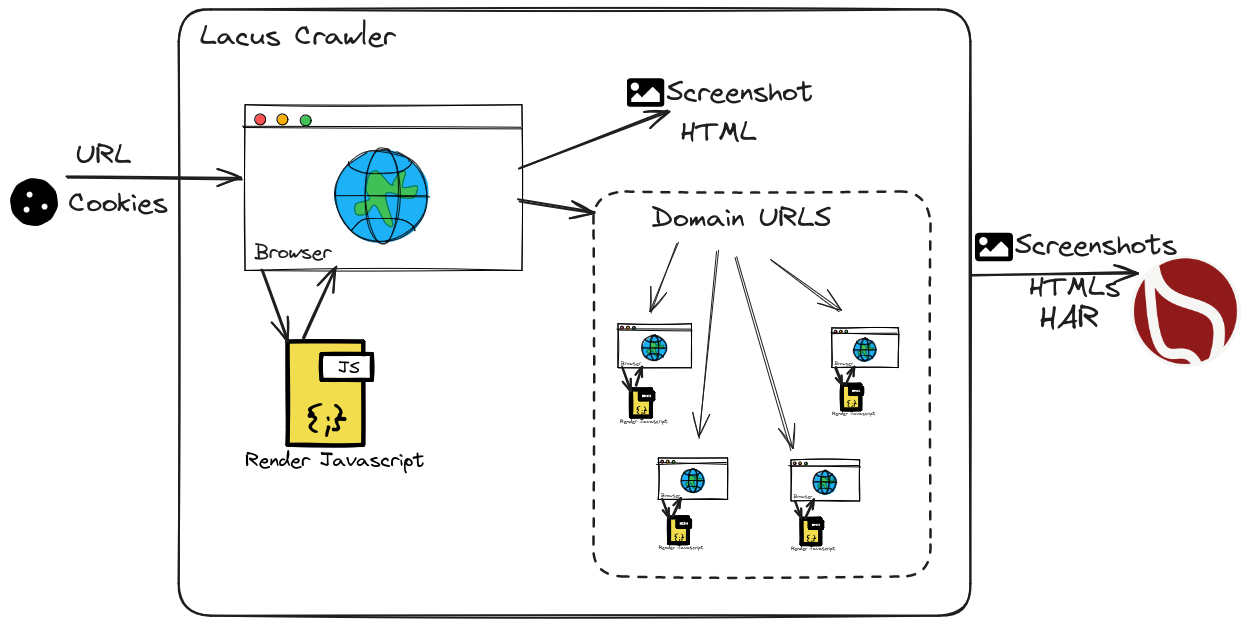
\includegraphics[scale=0.28]{images/ail-lacus.png}
    }
\end{frame}

\begin{frame}
        \frametitle {Crawler}
        \begin{itemize}
                \item Crawlers are used to navigate on regular website as well as .onion addresses (via automatic extraction of urls or manual submission)
                \item Lacus\footnote{\url{https://github.com/ail-project/lacus}} ("scriptable" browser) is rending the pages (including javascript) and produce screenshots (HAR archive too)
                \item How a domain is crawled by default:
		\begin{enumerate}
		    \item Fetch the first url
            \item Render javascript (webkit browser)
		    \item Extract all urls
		    \item Filter url: keep all url of this domain
		    \item crawl next url (max depth = 1)
		\end{enumerate}
        \end{itemize}
\end{frame}

\begin{frame}
    \frametitle{Lacus}
    	\begin{itemize}
            \item Lacus\footnote{\url{https://github.com/ail-project/lacus}} is a capturing system using playwright, as a web service
		    \item AIL utilizes Lacus for fetching and rendering domains.
			\begin{itemize}
				\item Lacus can be installed and executed outside of AIL,
				\item Enqueue what you want to capture,
				\item Trigger the capture,
				\item Get the capture result,
			\end{itemize}
        \end{itemize}
\end{frame}

\begin{frame}
	\frametitle{Crawler Settings - Lacus}
		\begin{figure}
		    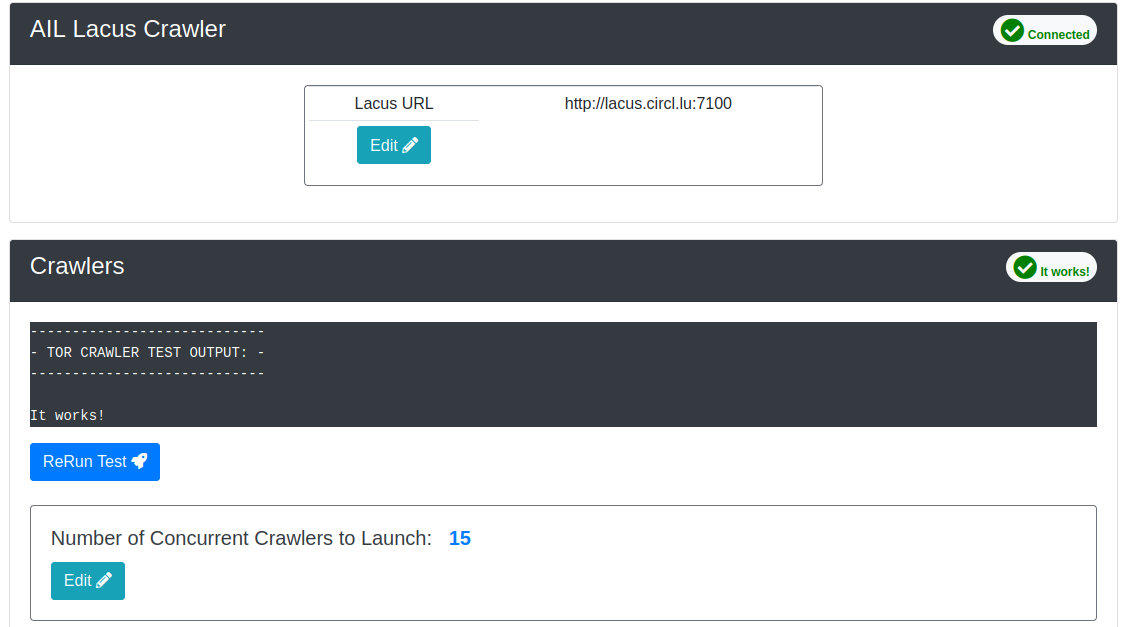
\includegraphics[scale=0.28]{screenshot/crawler_settings.png}
		\end{figure}
\end{frame}

\begin{frame}
    \frametitle{Crawler: Cookiejar}
    Use your cookies to login and bypass captcha
    \centerline{
        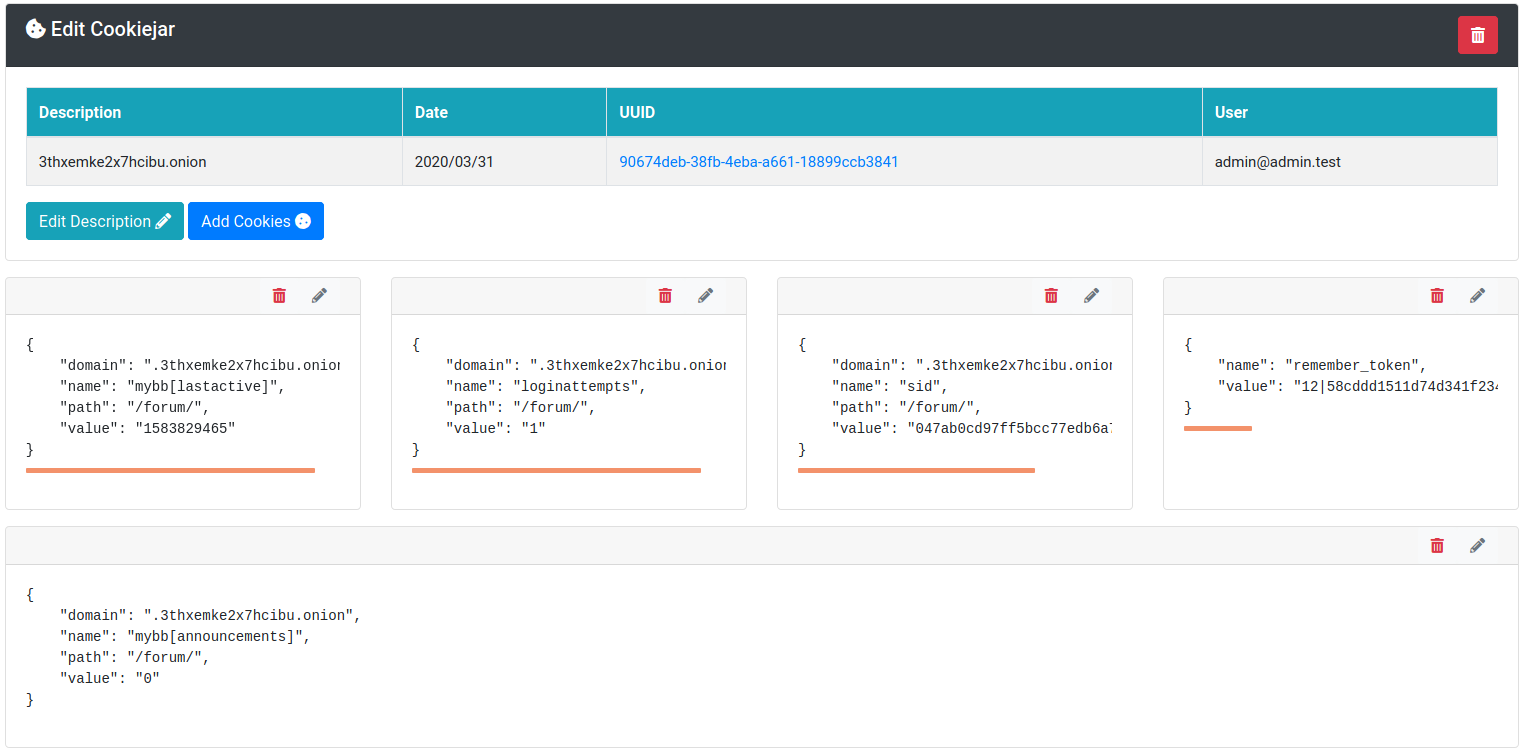
\includegraphics[scale=0.23]{screenshot/crawler-cookiejar-edit.png}
    }
\end{frame}

\begin{frame}
    \frametitle{Crawler: Cookiejar}
    \centerline{
        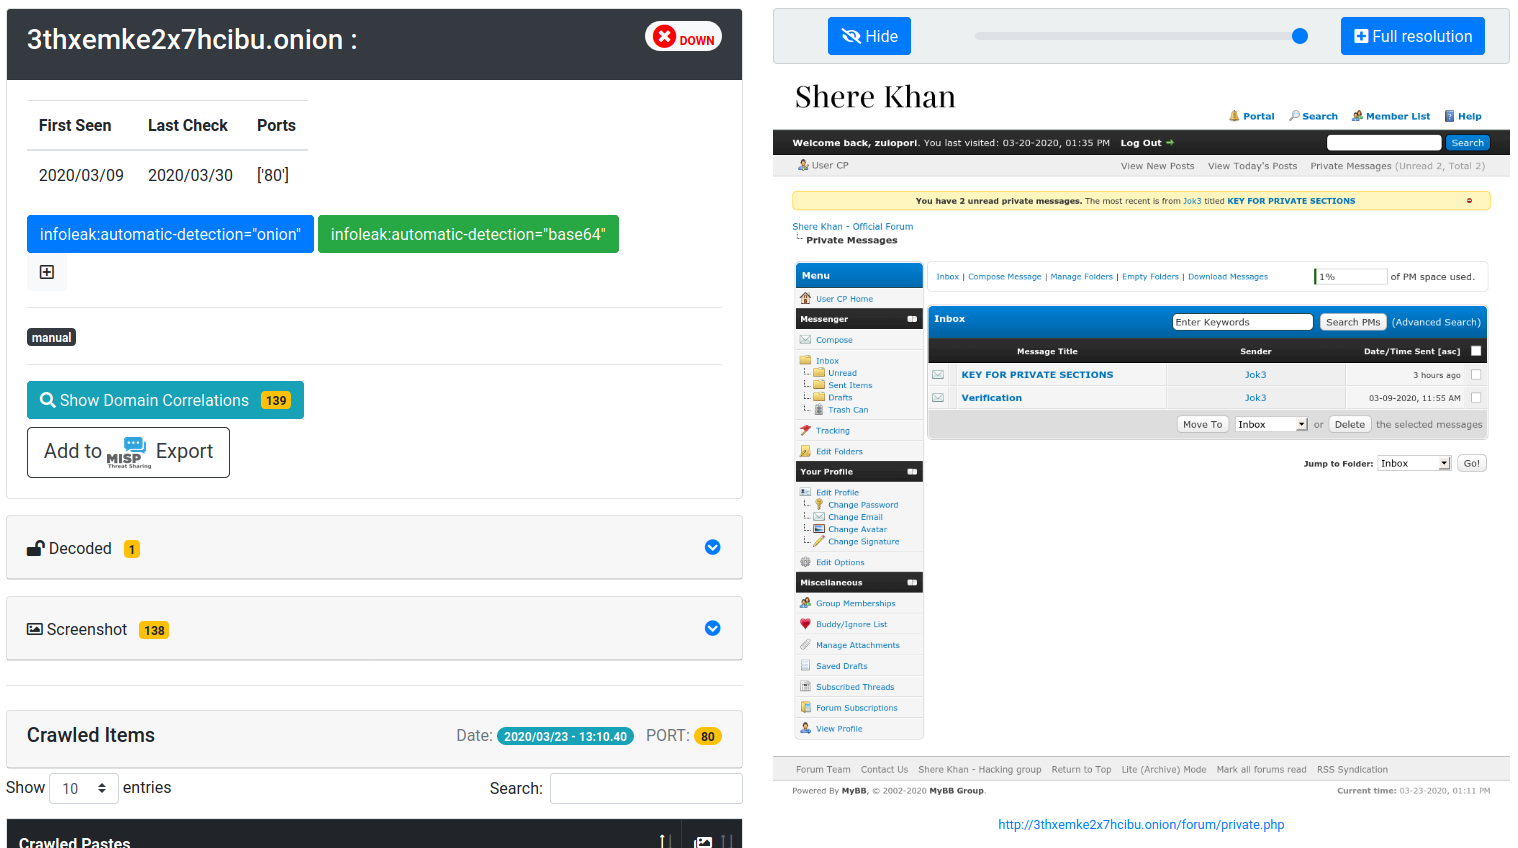
\includegraphics[scale=0.23]{screenshot/crawler-cookiejar-domain-crawled.png}
    }
\end{frame}

\section{Live demo!}

\begin{frame}
    \frametitle{Crawler: DDoS Booter}
    \centerline{
        \includegraphics[scale=0.23]{images/crawled-ddos.png}
    }
\end{frame}

\begin{frame}
    \frametitle{Correlations and relationship}
    \begin{figure}
        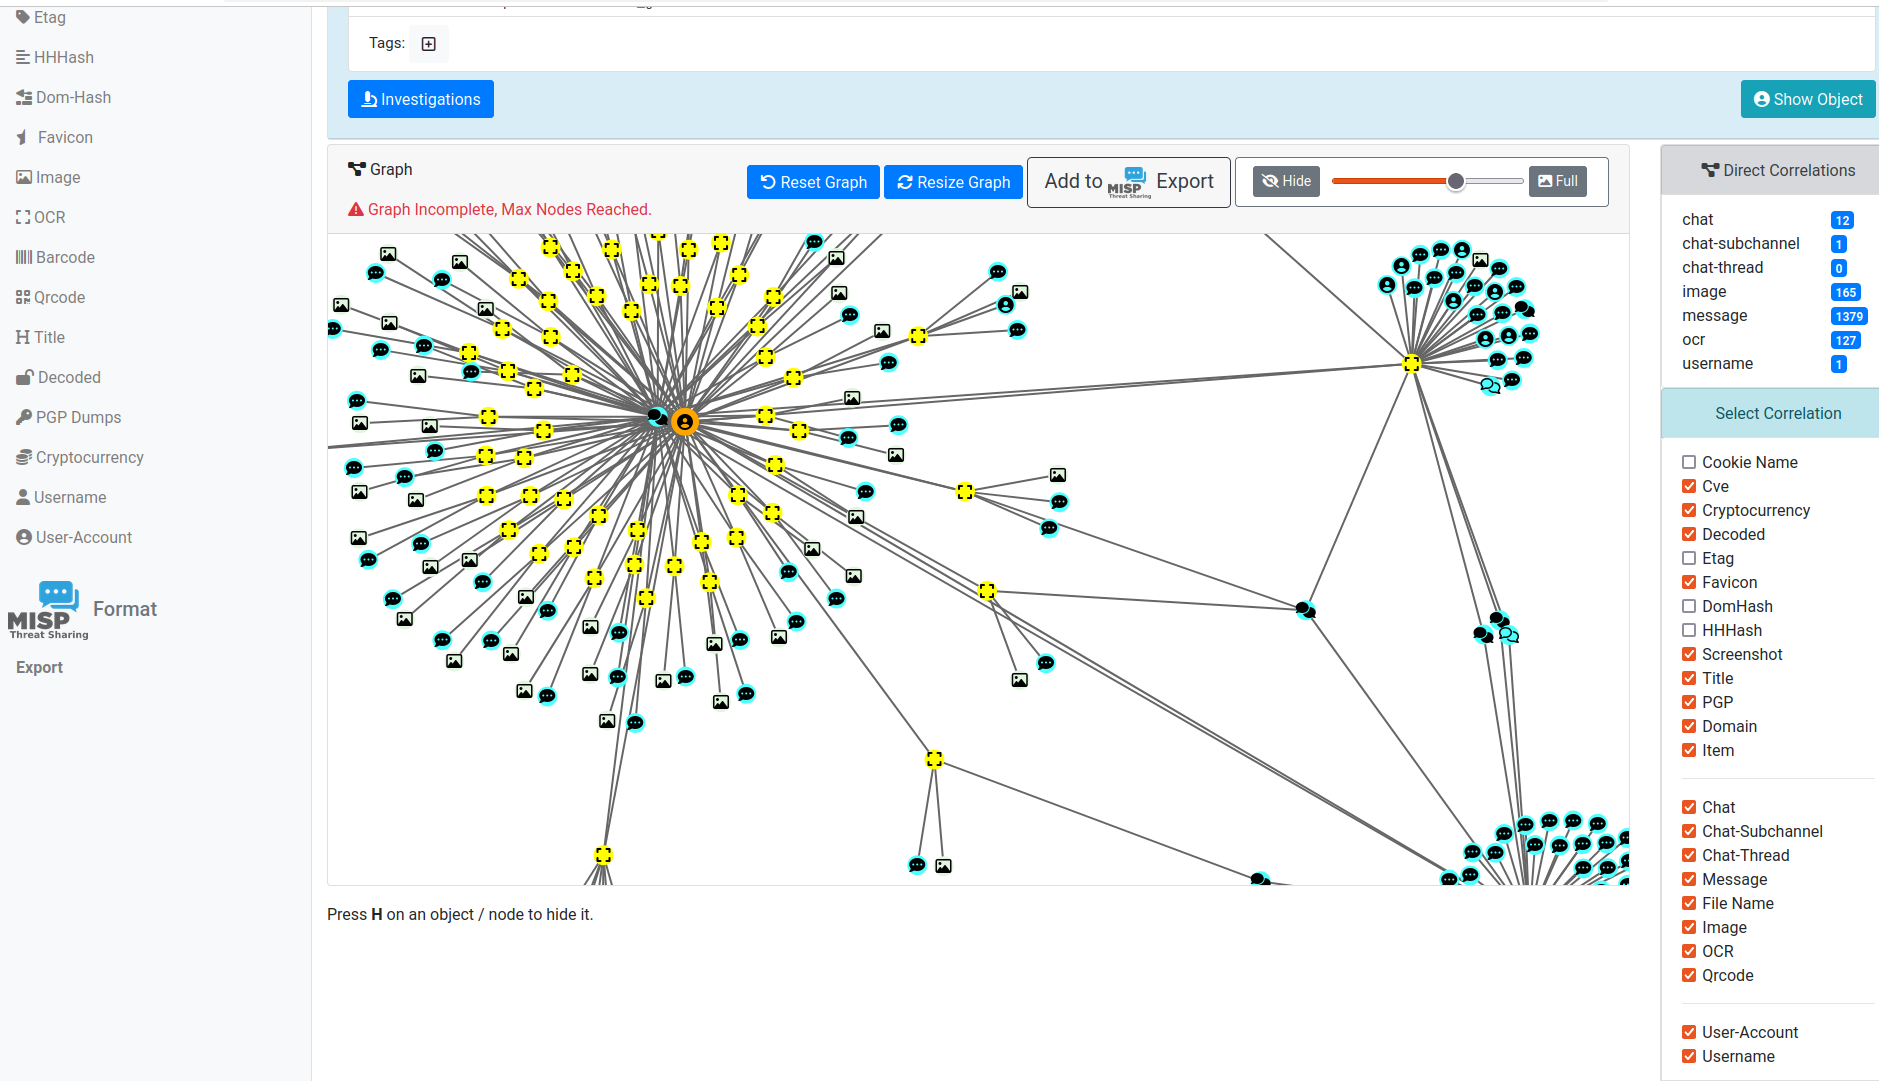
\includegraphics[scale=0.18, angle=0]{screenshot/correlation.png}
    \end{figure}
\end{frame}

\begin{frame}
    \frametitle{Investigations}
    \begin{figure}
        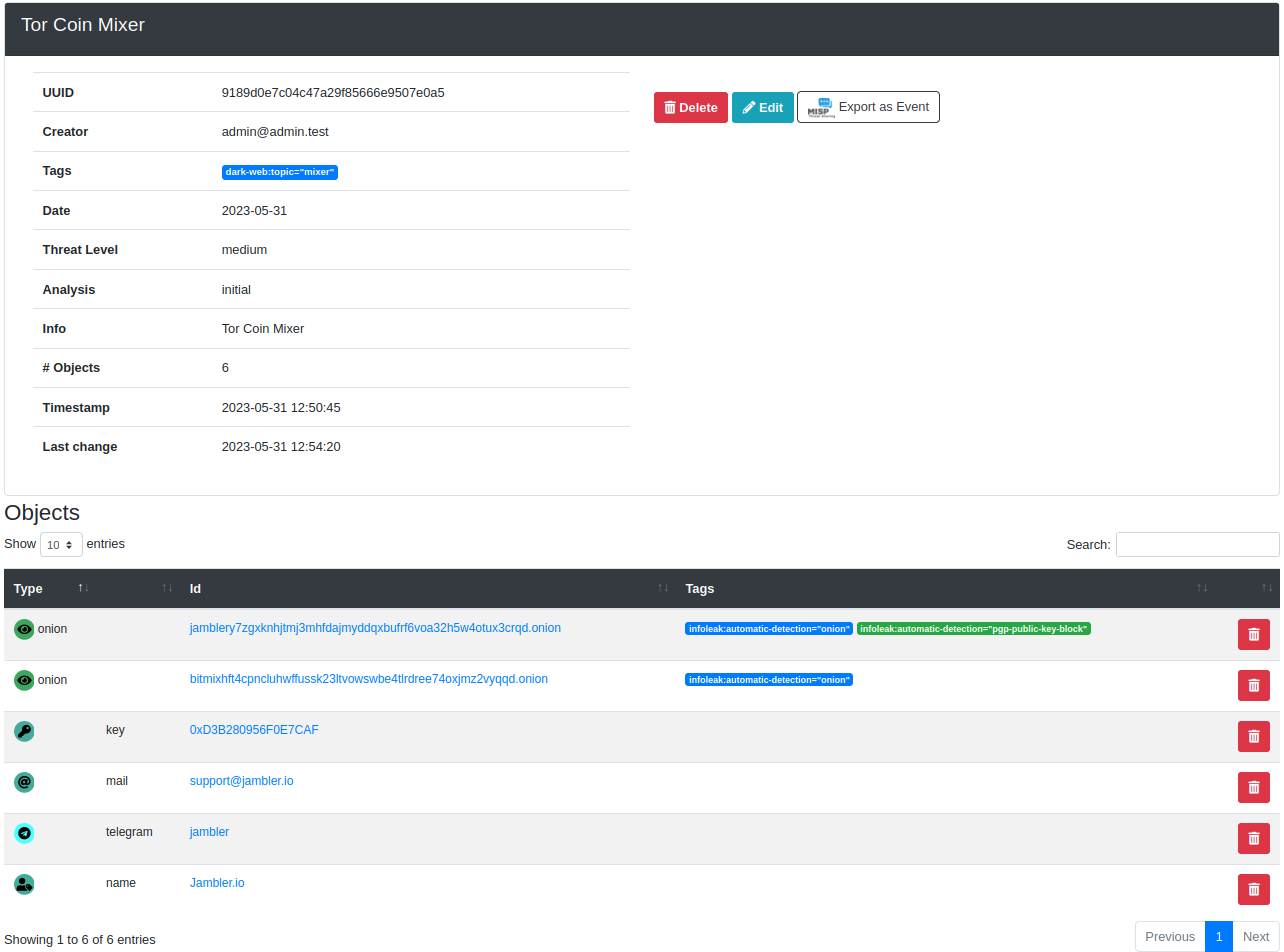
\includegraphics[scale=0.22, angle=0]{screenshot/investigation_mixer.png}
    \end{figure}
\end{frame}

% -> screenshot + user + images +
% \begin{frame}
%     \frametitle{Chats Monitoring}
%     \begin{figure}
%         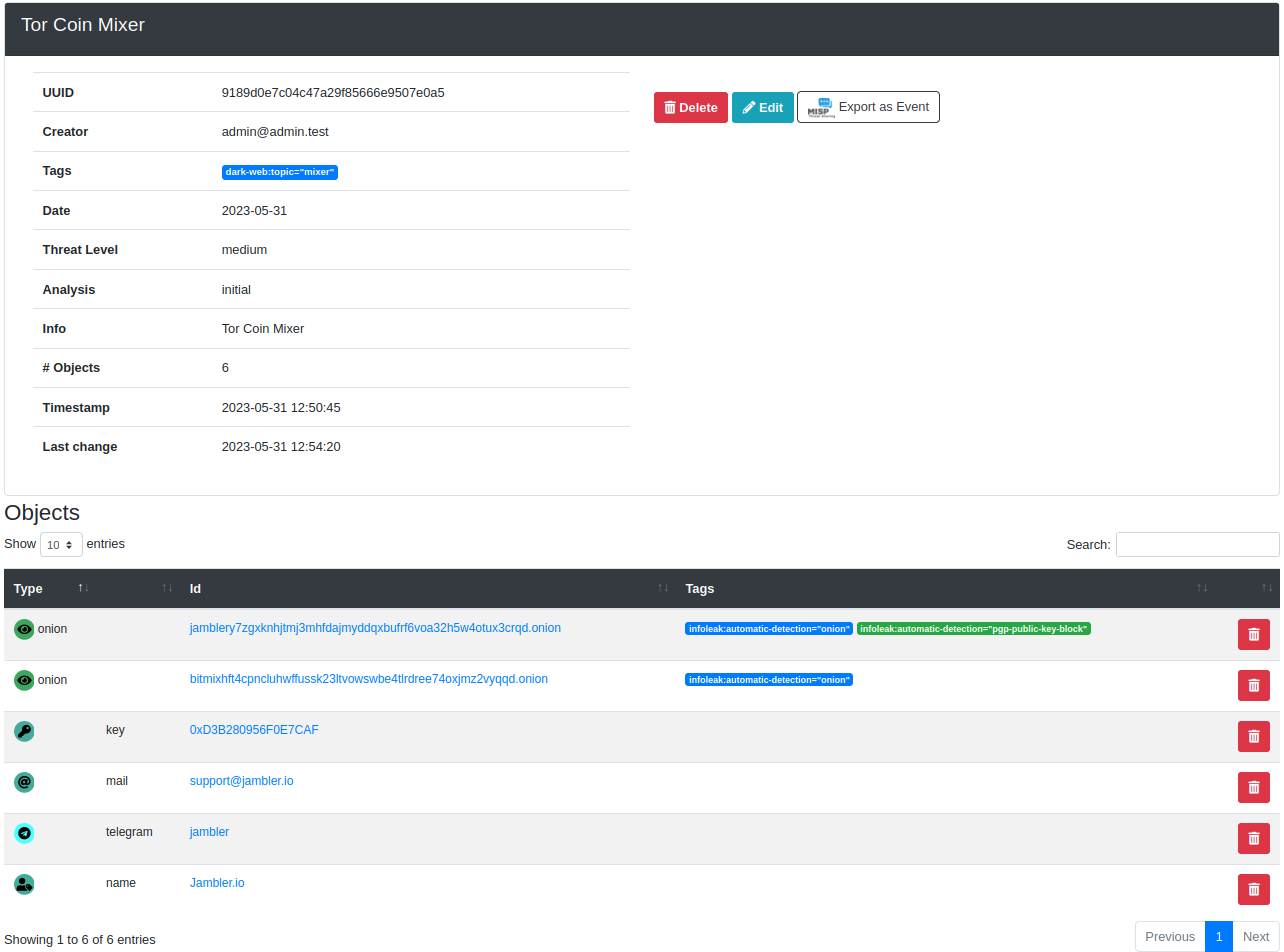
\includegraphics[scale=0.22, angle=0]{screenshot/investigation_mixer.png}
%     \end{figure}
% \end{frame}


\begin{frame}
    \frametitle{Dashboard}
    \begin{figure}
        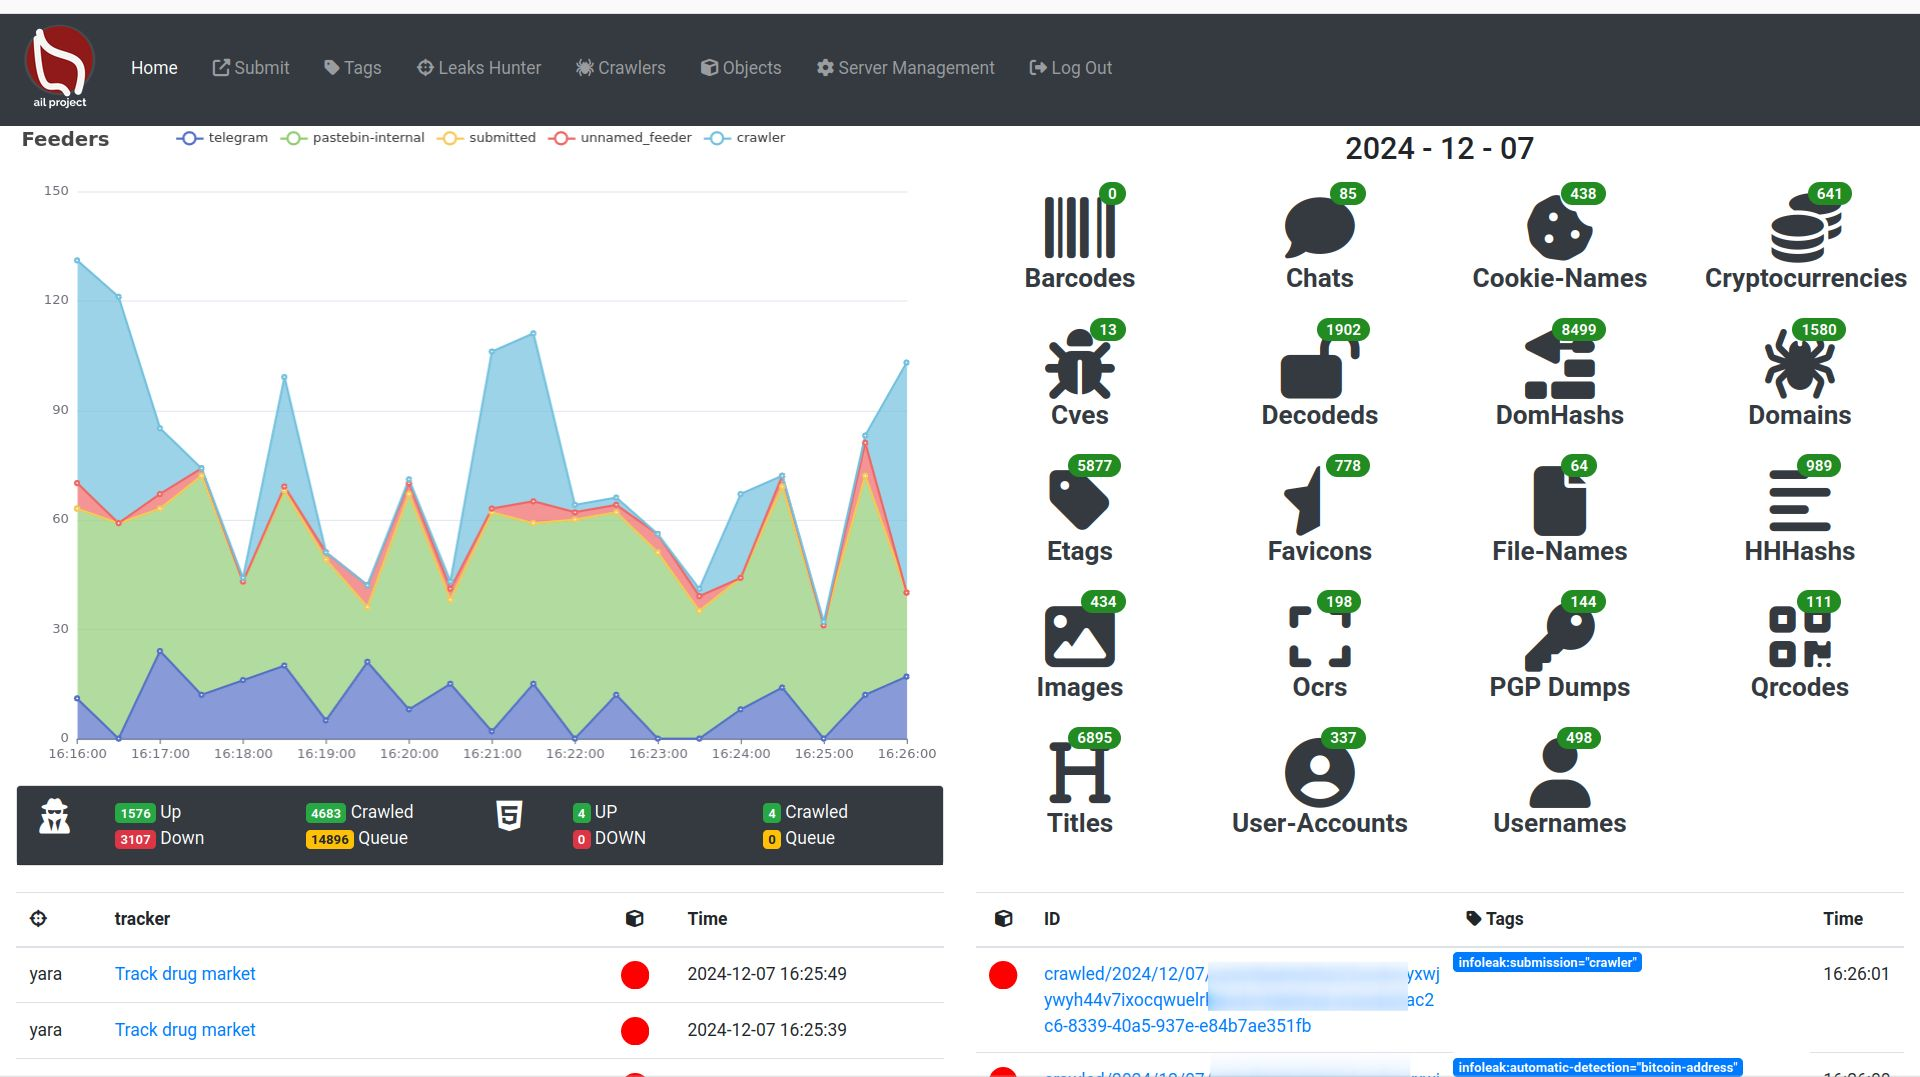
\includegraphics[scale=0.18, angle=0]{screenshot/dashboard.jpeg}
    \end{figure}
\end{frame}

\begin{frame}
    \frametitle{Example: Items Extracted}
    \begin{figure}
        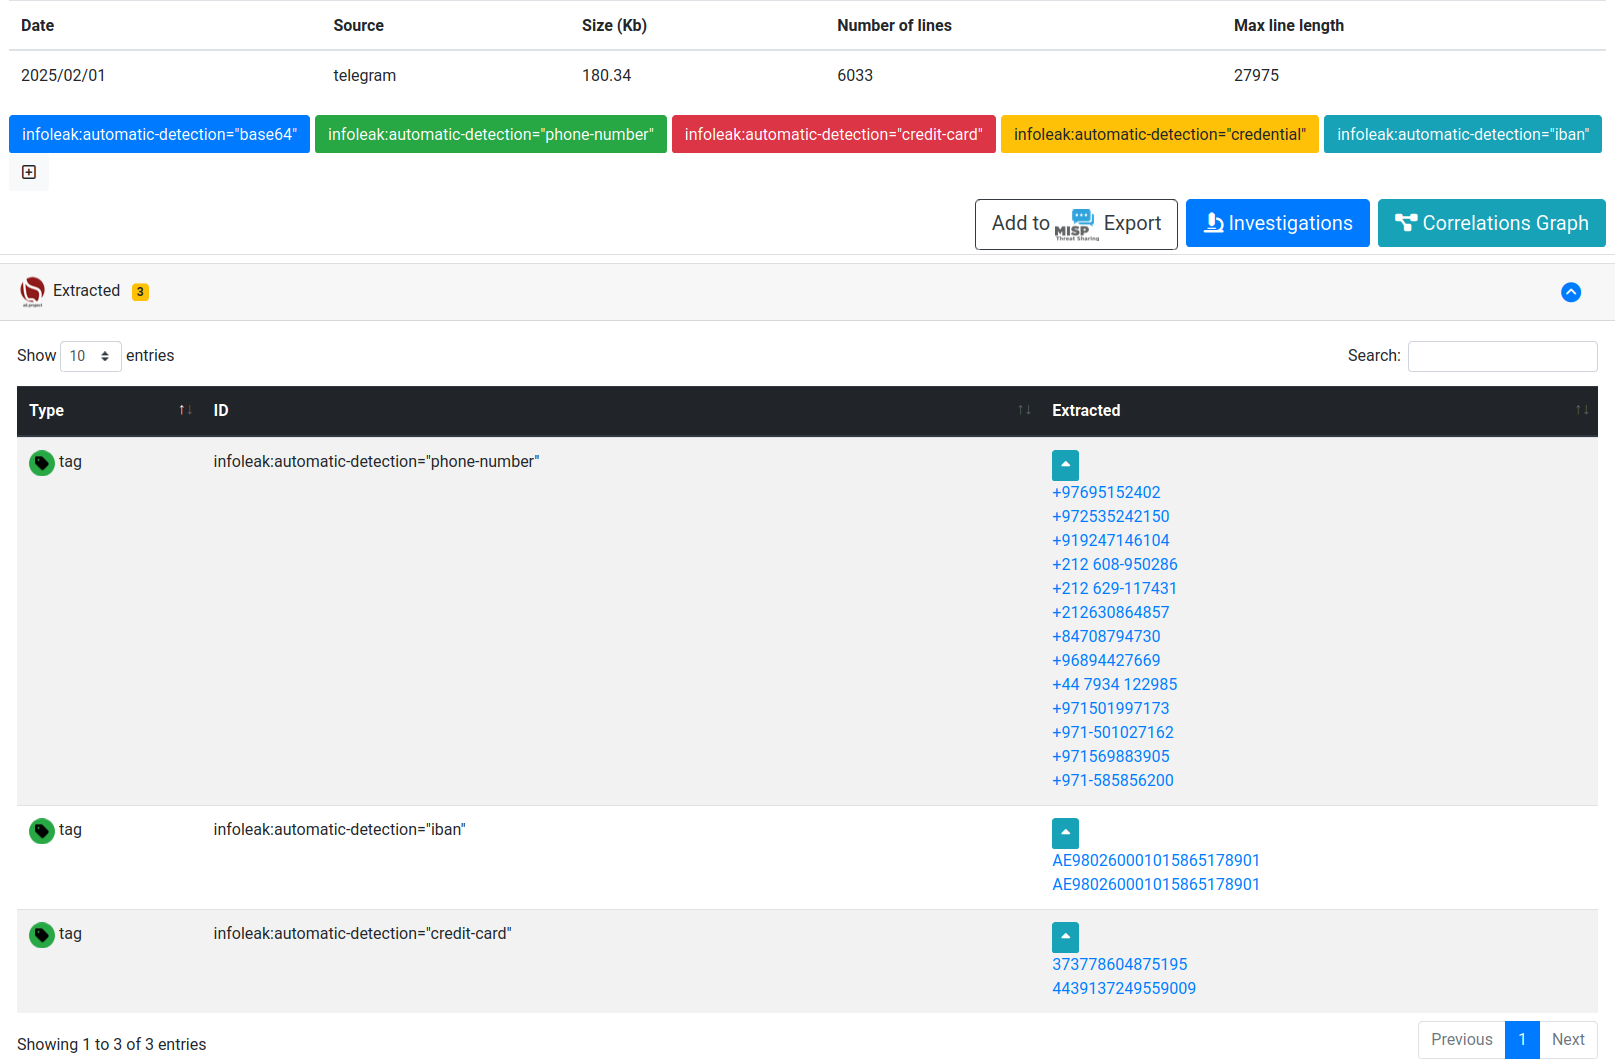
\includegraphics[scale=0.20, angle=0]{screenshot/item_meta.png}
    \end{figure}
\end{frame}

\begin{frame}
    \frametitle{Example: Items Domain}
    \begin{figure}
        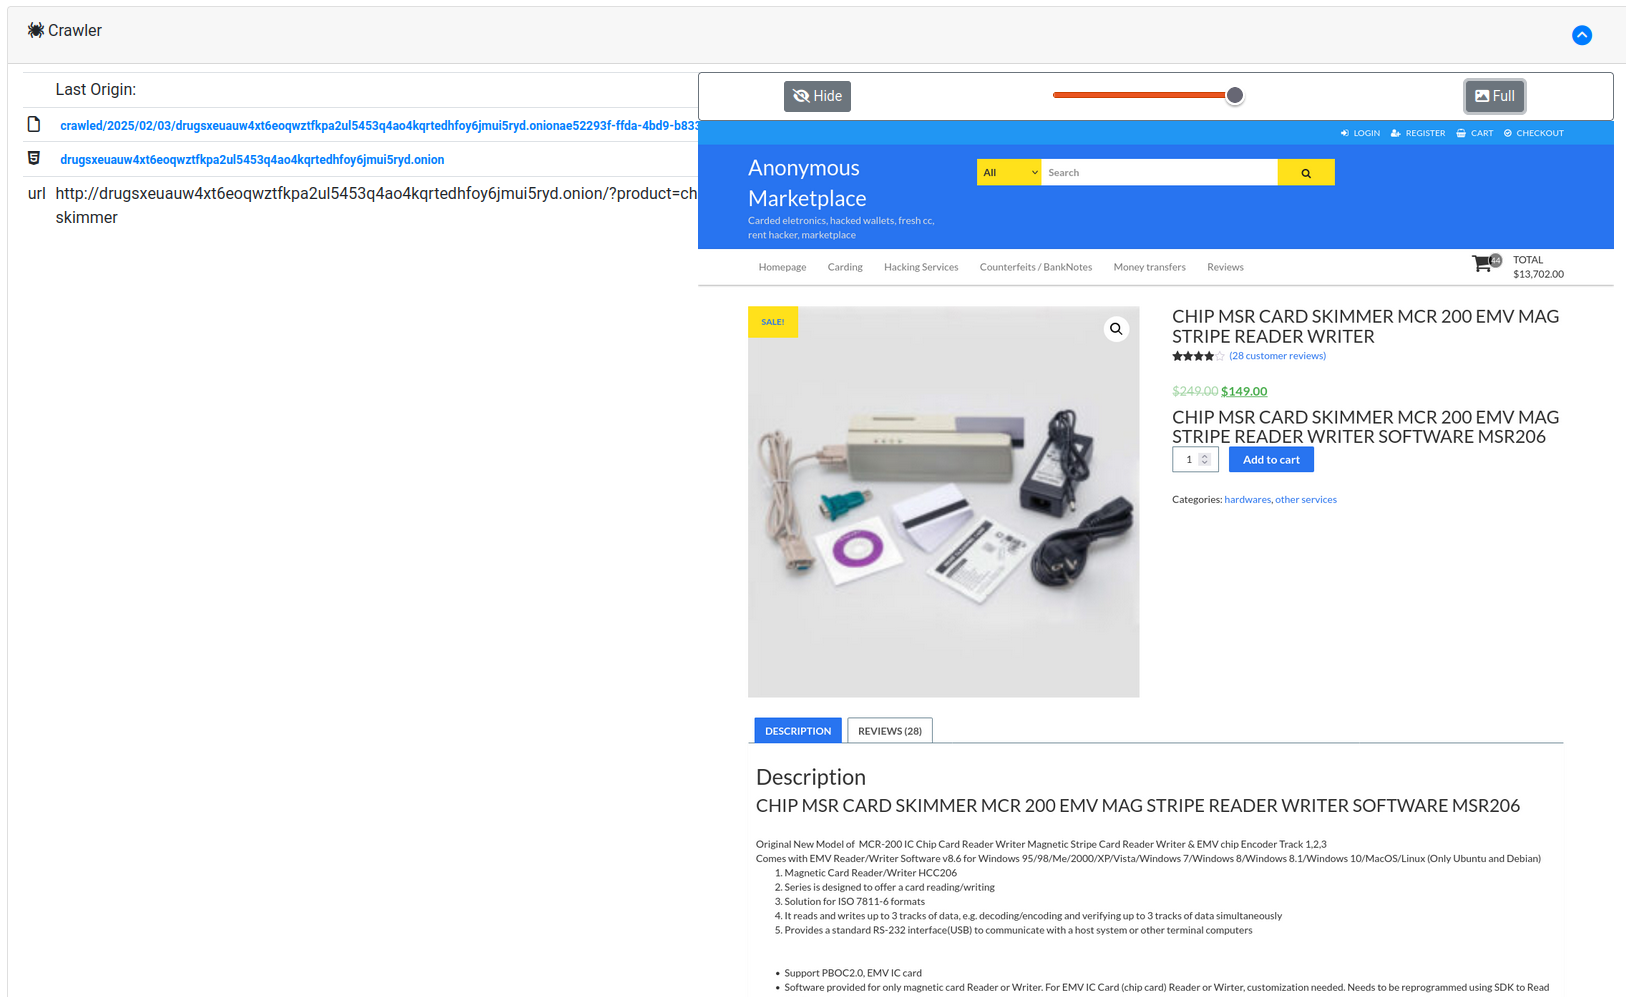
\includegraphics[scale=0.22, angle=0]{screenshot/item_domain.png}
    \end{figure}
\end{frame}

\begin{frame}
    \frametitle{Example: Browsing content}
    \begin{figure}
        \includegraphics[scale=0.3, angle=0]{images/ail_06.png}
    \end{figure}
\end{frame}

\begin{frame}
    \frametitle{Example: Search by tags}
    \begin{figure}
        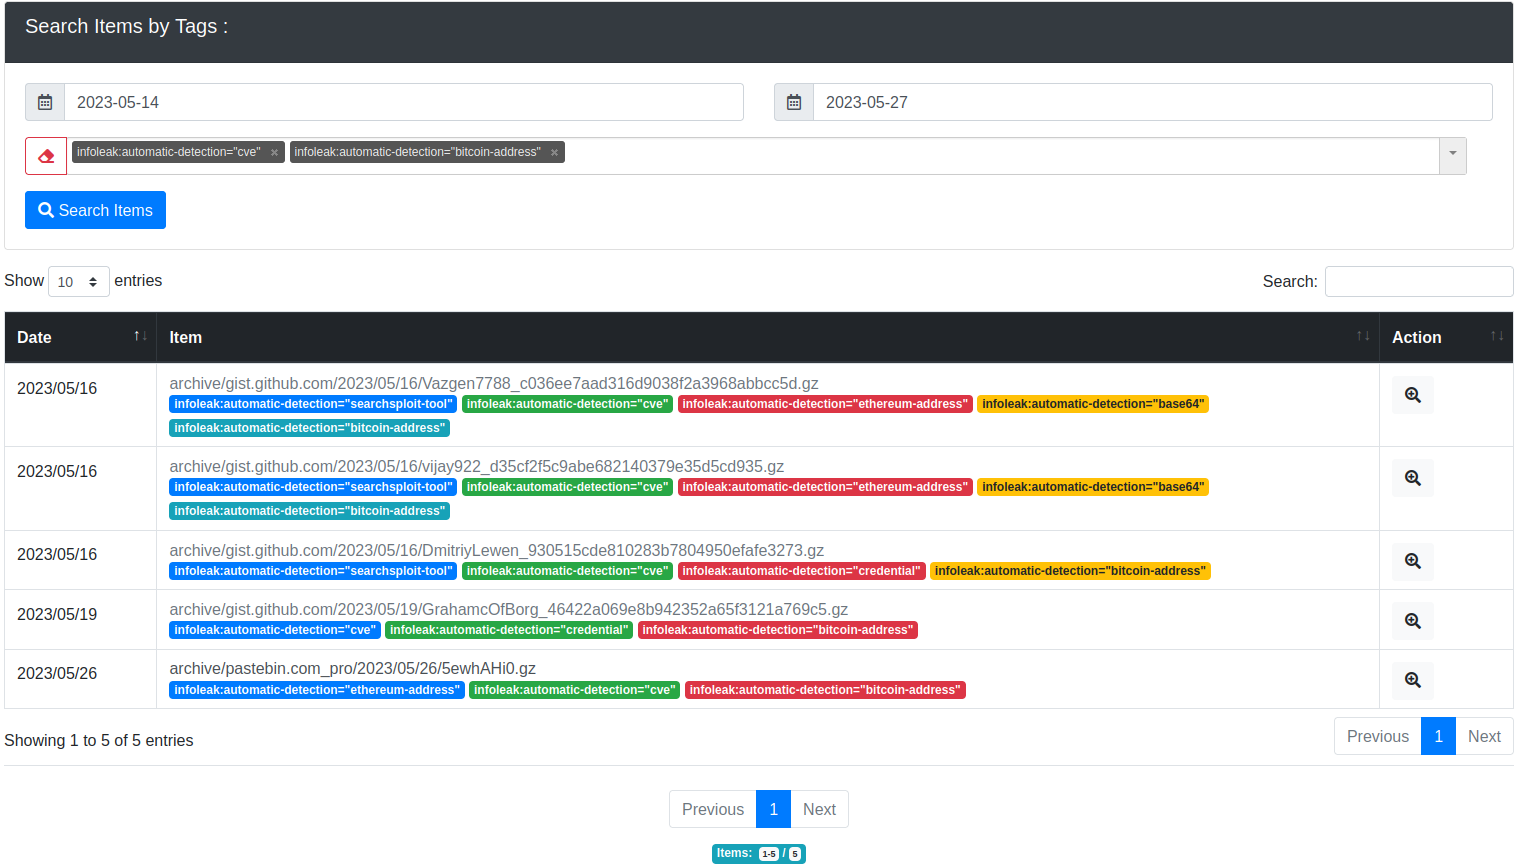
\includegraphics[scale=0.22, angle=0]{screenshot/tags_search_items.png}
    \end{figure}
\end{frame}
\section{MISP}

\begin{frame}
    \frametitle{MISP Taxonomies}
        \begin{itemize}
            \item {\bf Tagging} is a simple way to attach a classification to an event or attribute.
            \item {\bf Classification must be globally used to be efficient.}
            \item Provide a set of already defined classifications modeling estimative language
            \item Taxonomies are implemented in a simple JSON format \footnote{\url{https://github.com/MISP/misp-taxonomies}}.
            \item Can be easily cherry-picked or extended
        \end{itemize}
\end{frame}

\begin{frame}
    \frametitle{Taxonomies useful in AIL}
        \begin{itemize}
            \item {\bf infoleak}: Information classified as being potential leak.
            \item {\bf estimative-language}: Describe quality and credibility of underlying sources, data, and methodologies.
            \item {\bf admiralty-scale}: Rank the reliability of a source and the credibility of an information
            \item {\bf fpf\footnote{Future of Privacy Forum}}: Evaluate the degree of identifiability of personal data and the types of pseudonymous data, de-identified data and anonymous data.
        \end{itemize}
\end{frame}

\begin{frame}
    \frametitle{Taxonomies useful in AIL}
        \begin{itemize}
            \item {\bf tor}: Describe Tor network infrastructure.
            \item {\bf dark-web}: Criminal motivation on the dark web.
            \item {\bf copine-scale\footnote{Combating Paedophile Information Networks in Europe}}: Categorise the severity of images of child sex abuse.
        \end{itemize}
\end{frame}

\begin{frame}
    \frametitle{threat sharing and incident response platforms}
    \centerline{
        
\includegraphics[scale=0.14]{images/ail-project.png}
        \hskip 2em 
        $\longrightarrow$
        \hskip 2em
        \includegraphics[scale=0.8]{images/MISP.png}
    }

    \vskip 2em
    \textbf{Goal:} submission to threat sharing and incident
response platforms.
\end{frame}

\begin{frame}
    \frametitle{threat sharing and incident response platforms}
    \centerline{
        
\includegraphics[scale=0.12]{images/ail-project.png}
        \hskip 2em
        $\longrightarrow$
        \hskip 2em
        \includegraphics[scale=0.8]{images/MISP.png}
    }

    \vskip 2em
    \begin{enumerate}
            \item Use infoleak taxonomy\footnote{\url{https://www.misp-project.org/taxonomies.html}}
        \item Add your own tags
	\item Export AIL objects to MISP core format
	\item Download it or Create a MISP Event\footnote{\url{https://www.misp-standard.org/rfc/misp-standard-core.txt}}
    \end{enumerate}
\end{frame}

\begin{frame}
    \frametitle{MISP Export}
    \centerline{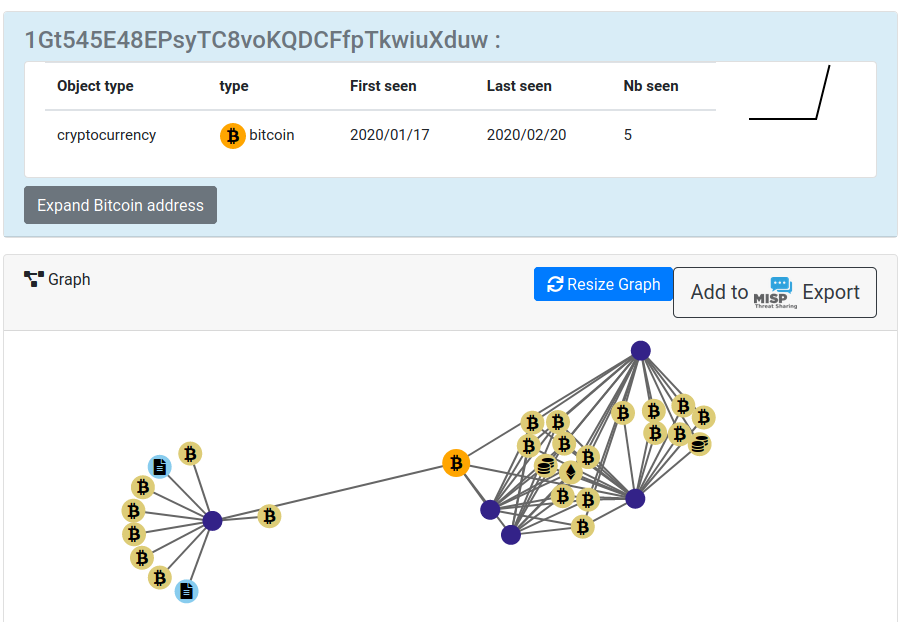
\includegraphics[scale=0.35]{screenshot/bitcoin-misp.png}}
\end{frame}

\begin{frame}
    \frametitle{MISP Export}
    \centerline{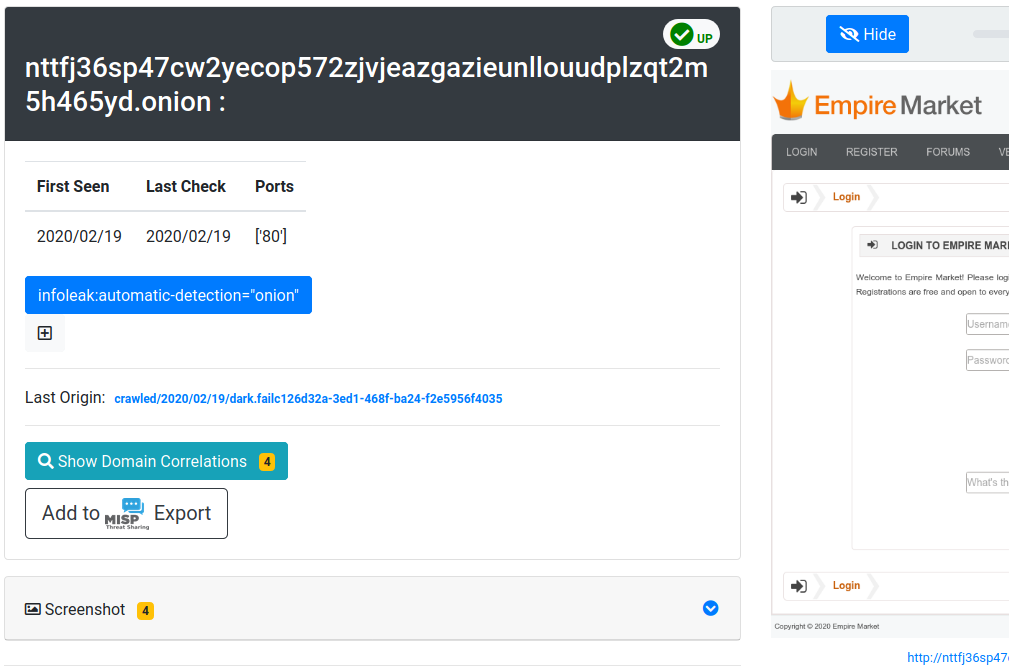
\includegraphics[scale=0.35]{screenshot/domain-misp.png}}
\end{frame}

\begin{frame}
    \frametitle{MISP Export}
    \centerline{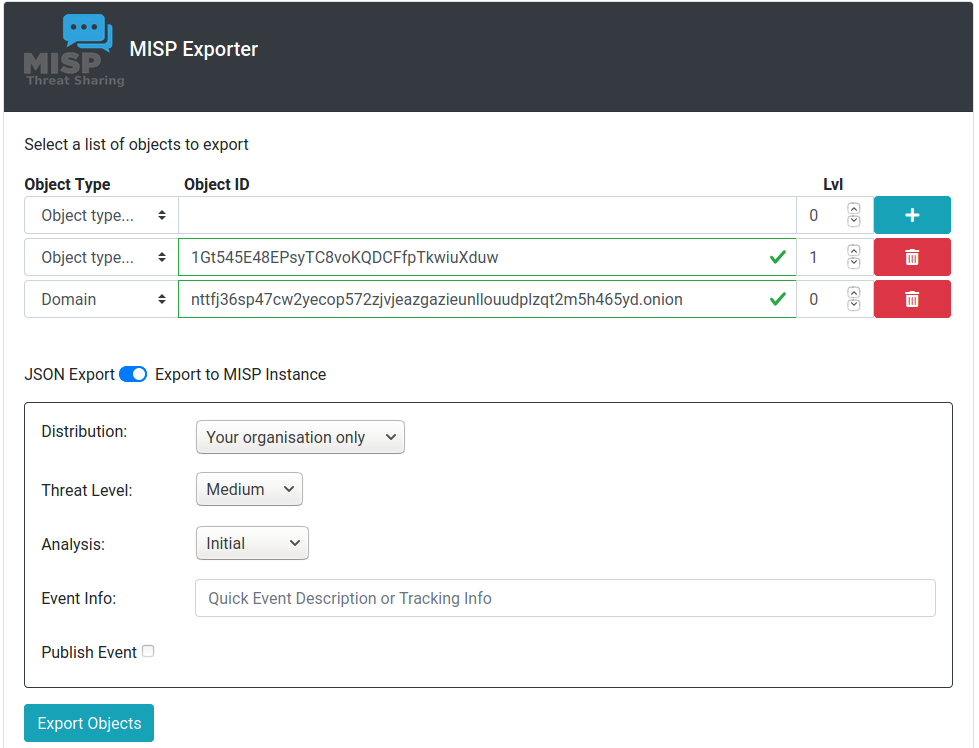
\includegraphics[scale=0.25]{screenshot/misp-export.png}}
\end{frame}

\begin{frame}
    \frametitle{Automatic MISP Export on tags}
    \centerline{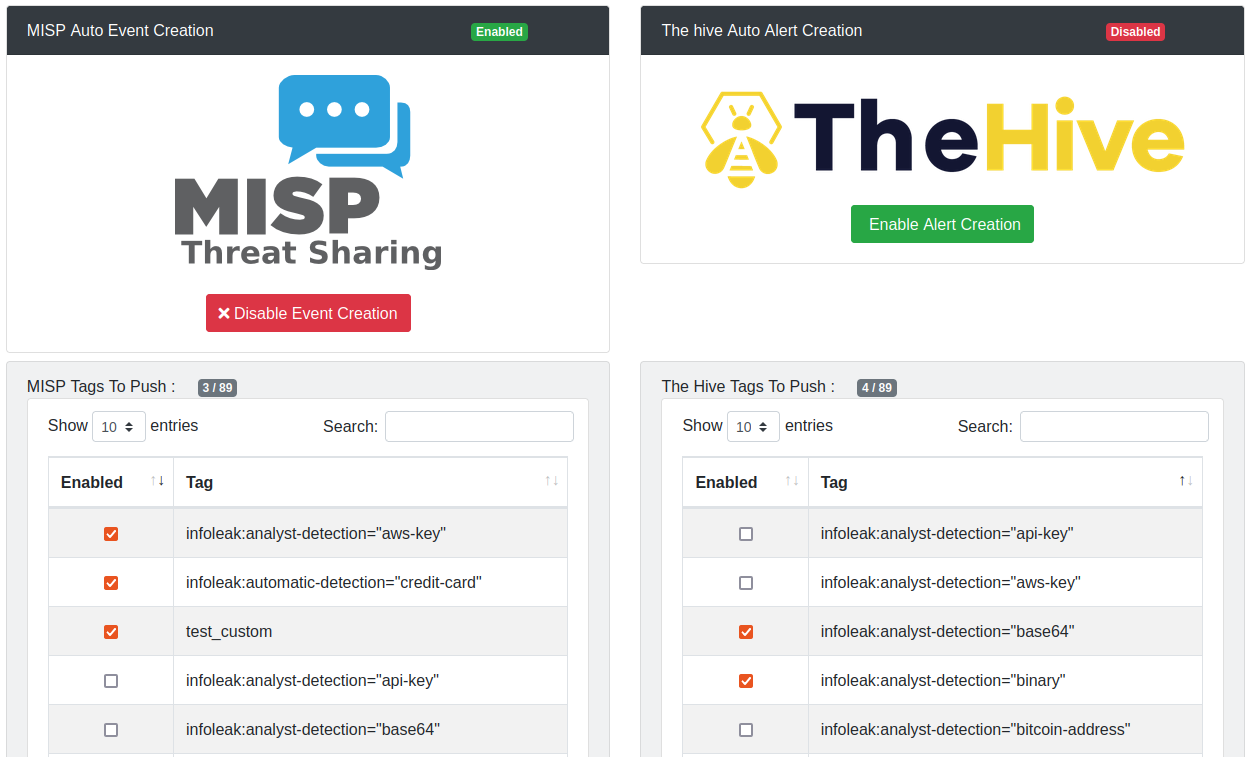
\includegraphics[scale=0.25]{screenshot/tags_misp_auto.png}}
\end{frame}


\section{API}

\begin{frame}[fragile]
AIL exposes a ReST API which can be used to interact with the back-end\footnote{\url{https://github.com/ail-project/ail-framework/blob/master/doc/README.md}}.

        \begin{lstlisting}
curl https://127.0.0.1:7000/api/v1/add/crawler/task
        --header "Authorization: iHc1_ChZxj1aXmiFiF1mkxxQkzawwriEaZpPqyTQj"
        -H "Content-Type: application/json"
        --data @input.json -X POST
        \end{lstlisting}
%         \begin{itemize}
%                 \item AIL API is currently covering 60\% of the functionality of back-end.
%         \end{itemize}
\end{frame}

\section{Setting up the framework}
\lstset{style=bash}
\begin{frame}[fragile]
    \frametitle{Setting up AIL-Framework from source}
    \begin{tcblisting}{colback=black!85,coltext=green,listing only,
        title=Setting up AIL-Framework from source, fonttitle=\bfseries}
git clone https://github.com/ail-project/ail-framework.git
cd AIL-framework
./installing_deps.sh
\end{tcblisting}
\end{frame}

%IMPORTERS
\section{Feeding the framework}

\begin{frame}
\frametitle{Feeding Data to AIL}
    There are different ways to feed data into AIL:
    \begin{enumerate}
        \item AIL Importers:
            \begin{itemize}
                \item Dir / Files
                \item ZMQ
                % \item Be a trusted partner with CIRCL and ask to get access to our zmq feed {\tiny \href{mailto:info@circl.lu}{info@circl.lu}}
                \item \textit{pystemon}
            \end{itemize}
        \item AIL Feeders (discord, telegram, ...)
        \item Feed your own data using the API
        \item Feed your own file/text using the UI (\texttt{Submit section})
    \end{enumerate}
\end{frame}

\begin{frame}
    \frametitle{Feeding Data to AIL - Limitation}
    \centerline{\includegraphics[scale=0.1]{images/alert.png}}
    \alert{/!$\backslash$ Limitation:}
    \vskip 1em
    \begin{itemize}
        \item Each file to be fed must be of a reasonable size:
        \begin{itemize}
            \item \texttt{$\sim$ 3 Mb /} file is already large
            \item This is because some modules are doing regex matching (default timeout of 30 seconds)
            \item If you want to feed a large file, better split it in multiple ones
        \end{itemize}

    \end{itemize}
\end{frame}

\subsection{UI}

\begin{frame}
    \frametitle{Via the UI (1)}
    \centerline{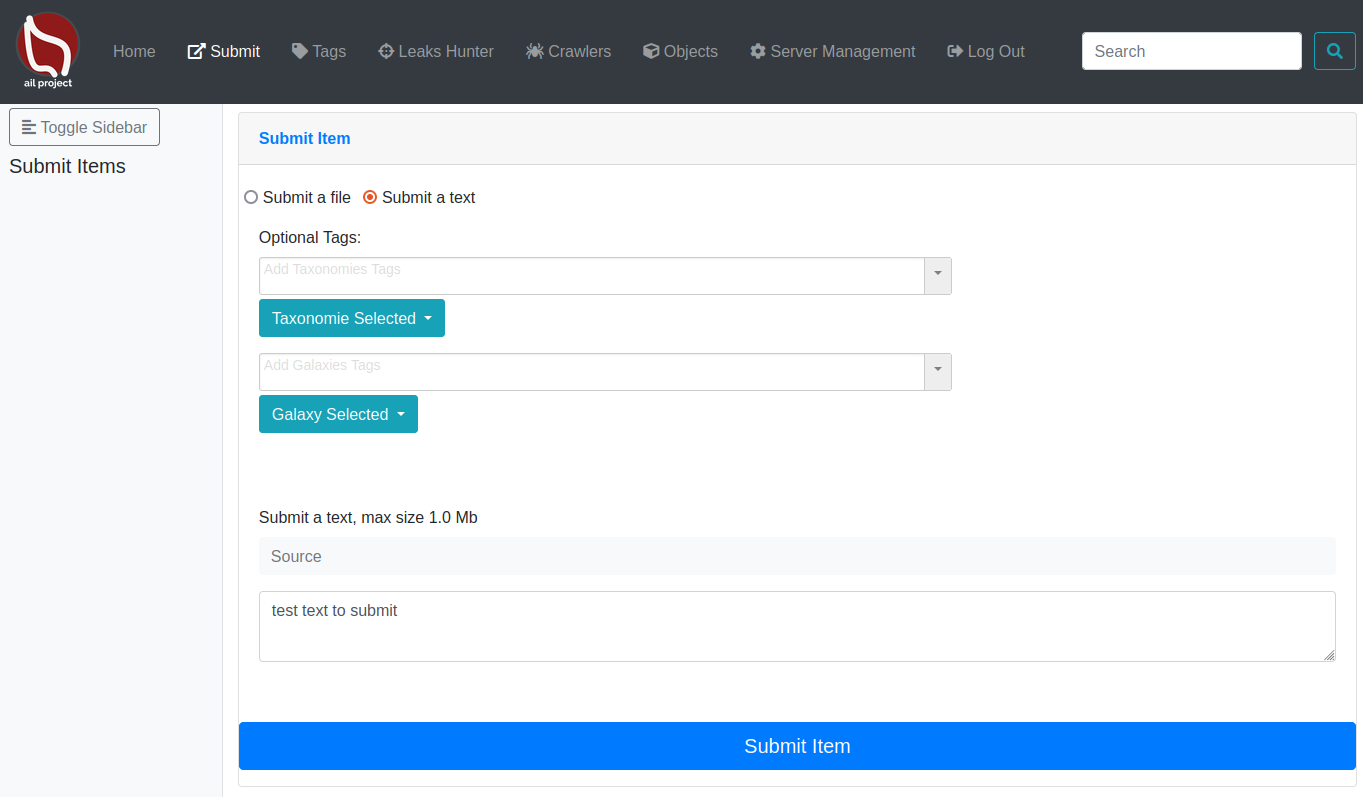
\includegraphics[scale=0.20]{screenshot/ui_submit.png}}
\end{frame}

\begin{frame}
    \frametitle{Via the UI (2)}
    \centerline{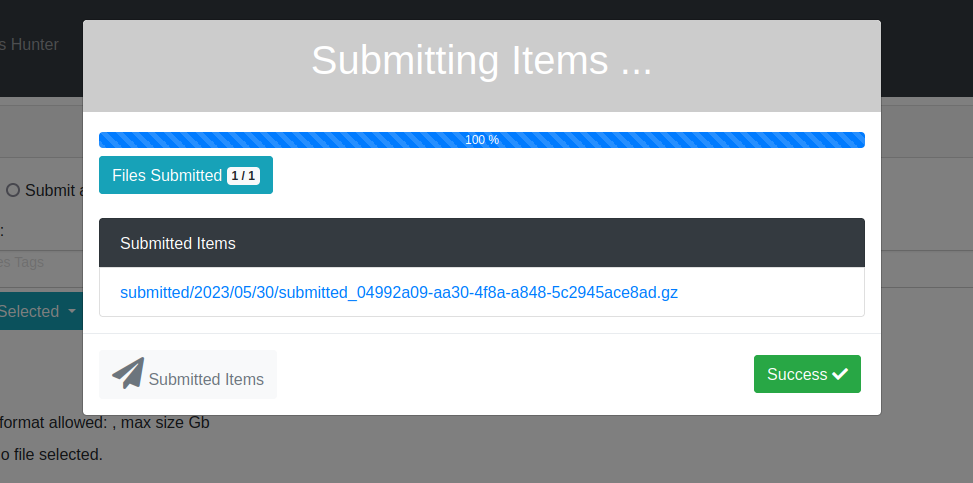
\includegraphics[scale=0.29]{screenshot/ui_submit0.png}}
\end{frame}

\subsection{API}

\begin{frame}[fragile]
    \frametitle{API - Feeding AIL with your own data}
    \begin{tcblisting}{colback=black!85,coltext=green,listing only,
        title=api/v1/import/item, fonttitle=\bfseries}
{
  "type": "text",
  "tags": [
    "infoleak:analyst-detection=\"private-key\""
  ],
  "text": "text to import"
}
\end{tcblisting}
 
\end{frame}

\subsection{Importers}

\begin{frame}
    \frametitle{Importers}
    \begin{itemize}
        \item Importers are located in the \texttt{/bin/importer} directory
        \item They are used to import different types of data into AIL
        \item Adding new Importers is straightforward.
        \item Available Importers:
            \begin{itemize}
                \item AIL Feeders
                \item ZMQ
                \item pystemon
                \item Files
            \end{itemize}
    \end{itemize}
\end{frame}

% ZMQ
% Pystemon

\lstset{style=bash}
\begin{frame}[fragile]
    \frametitle{File Importer}
    \begin{itemize}
        \item \texttt{importer/FileImporter.py}
    \end{itemize}
    \begin{tcblisting}{colback=black!85,coltext=green,listing only,
        title=Import File, fonttitle=\bfseries}
. ./AILENV/bin/activate
cd tools/
./file_dir_importer.py -f MY_FILE_PATH
    \end{tcblisting}
    \begin{tcblisting}{colback=black!85,coltext=green,listing only,
        title=Import Dir, fonttitle=\bfseries}
. ./AILENV/bin/activate
cd tools/
./file_dir_importer.py -d MY_DIR_PATH
    \end{tcblisting}
\end{frame}


\subsubsection{AIL Feeders}

\begin{frame}[fragile]
    \frametitle{AIL feeders Importers}
    \begin{itemize}
        \item {\bf 12+ feeders are available} for all AIL users to feed from external sources
        \item External feeders can run anywhere and are completely separated from AIL framework
        \item The feeder can use their {\bf own internal logic} and even push JSON metadata
        \item Feeder are then pushing the generated JSON to AIL API
    \end{itemize}
\end{frame}

% \begin{frame}[fragile]
%    \frametitle{Feeding AIL with Twitter posts and associated urls}
%         \begin{itemize}
%                 \item AIL - feeder from Twitter\footnote{\url{https://github.com/ail-project/ail-feeder-twitter}}
%                 \item The AIL-feeder-twitter {\bf search specific keywords on Twitter} using Twint (without API), crawls the urls and pushes the results in AIL
%                 \item The JSON format format can be extended via meta fields
%         \end{itemize}
% \end{frame}

\begin{frame}[fragile]
   \frametitle{Certificate transparency feeder for AIL}
    \begin{itemize}
        \item ail-feeder-cti\footnote{\url{https://github.com/ail-project/ail-feeder-ct}} is a generic software to extract information from a certstream server (certificate transparency)
        \item All metadata extracted will be processed by AIL
        \item Onion addresses crawled automatically by AIL if seen in a certificate 
    \end{itemize}
\end{frame}

\begin{frame}[fragile]
    \frametitle{GitHub archive and GitHub repository}
    \begin{itemize}
        \item ail-feeder-gharchive\footnote{\url{https://github.com/ail-project/ail-feeder-gharchive}} is a generic software to extract informations from {\bf GHArchive}, collect and feed AIL via AIL ReST API
        \item ail-feeder-github-repo\footnote{\url{https://github.com/ail-project/ail-feeder-github-repo}} is collecting from a GitHub repository and push everything to AIL
        \item For monitoring a set of {\bf suspicious git repositories} or finding leaks on existing or managed git repositories, it's a simple way to feed AIL with such source.
    \end{itemize}
\end{frame}

\begin{frame}[fragile]
    \frametitle{AIL LeakFeeder}
    \begin{itemize}
        \item ail-feeder-leak\footnote{\url{https://github.com/ail-project/ail-feeder-leak}} automates the process to feed leaked large files automatically to AIL
    \end{itemize}
    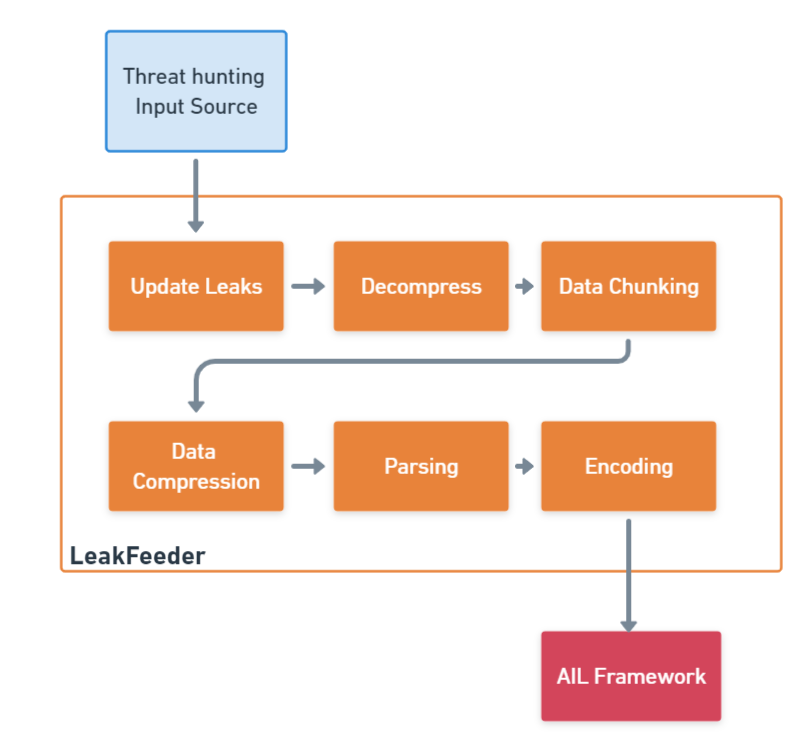
\includegraphics[scale=0.20]{./images/feeder_leak.png}
\end{frame}

\begin{frame}[fragile]
    \frametitle{AIL feeder ActivityPub}
    \begin{itemize}
        \item ail-feeder-activity-pub\footnote{\url{https://github.com/ail-project/ail-feeder-activity-pub}} is feeder for the ActivityPub standard used in distributed social networks
        \item Accounts are required on the ActivityPub instance to get the stream
    \end{itemize}
\end{frame}

\begin{frame}[fragile]
    \frametitle{AIL feeder telegram}
    \begin{itemize}
        \item ail-feeder-telegram\footnote{\url{https://github.com/ail-project/ail-feeder-telegram}} is a {\bf Telegram feeder}
        \item An API ID/hash for Telegram is required and linked to your Telegram phone number
    \end{itemize}
\end{frame}

\begin{frame}[fragile]
    \frametitle{More feeders}
    \begin{itemize}
        \item ail-feeder-discord\footnote{\url{https://github.com/ail-project/ail-feeder-discord}} is a generic {\bf Discord} feeder for AIL
        \item ail-feeder-atom-rss\footnote{\url{https://github.com/ail-project/ail-feeder-atom-rss}} is an {\bf Atom and RSS reader} and feeder for AIL   
        \item ail-feeder-jsonlogs\footnote{\url{https://github.com/ail-project/ail-feeder-jsonlogs}} is a {\bf JSON aggregator} to submit generic JSON input into AIL
    \end{itemize}
\end{frame}


%% CONTI leak example
\begin{frame}[fragile]
	\frametitle{Feeding AIL with custom JSON}
	\begin{figure}[t]
		
\includegraphics[width=.8\textwidth]{screenshot/contileaks-twitter.png}
		\centering
	\end{figure}

	\begin{figure}[t]
		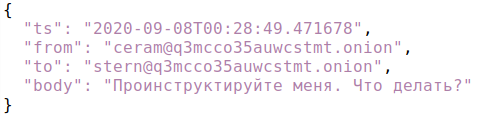
\includegraphics[width=.6\textwidth]{screenshot/contileaks-json.png}
		\centering
	\end{figure}

\end{frame}

\begin{frame}[fragile]                                                                                                                        

   \frametitle{Feeding AIL with Conti leaks}

        \begin{itemize}
		\item Conti jabber leaks are a good candidate for AIL analysis:
        	\begin{itemize}
			\item PGP keys
			\item Bitcoin addresses, maybe others,
			\item onion hidden services
        	\end{itemize}
        \item first we translated the files on english using deepl.com
		\item then we created a feeder to import json data in AIL
		\item Support added in AIL to correlate jabber usernames
        \end{itemize}

\end{frame}


\begin{frame}[fragile]                                                                                                                        
   \frametitle{Feeding AIL with Conti leaks}
	\lstinputlisting[language=Python]{feeder.py}

	\begin{lstlisting}[language=bash]
	$ cat ~/conti/* | jq . -c | python ./feeder.py
	\end{lstlisting}

\end{frame}

\begin{frame}[fragile]                                                                                                                        

\frametitle{Feeding AIL with Conti leaks}

    \begin{itemize}
    \item use grep to limit the noise on an instance by only sending interesting bits:
        \begin{itemize}
        \item PGP keys
\begin{lstlisting}[language=bash]
$ cat ~/conti/* | jq . -c | grep PGP | python ./feeder.py
\end{lstlisting}
        \item onion hidden services \texttt{| grep http:// |}
        \item telegram addresses \texttt{| grep tg:// | }
        \item bitcoins addresses \texttt{| egrep --regexp="[13][a-km-zA-HJ-NP-Z1-9]{25,34}" | }

        \end{itemize}
    \end{itemize}

\end{frame}


%STARTING THE SYSTEM
\section{Starting the framework}
\lstset{style=bash}
\begin{frame}[fragile]
    \frametitle{Running your own instance from source}
    \begin{tcblisting}{colback=black!85,coltext=green,listing only,
        title=Accessing the environment and starting AIL, fonttitle=\bfseries}

# Launch the system and the web interface
cd bin/
./LAUNCH -l

\end{tcblisting}
\end{frame}

\begin{frame}[fragile]
    \frametitle{Updating AIL}
    \begin{tcblisting}{colback=black!85,coltext=green,listing only,
        title=Launch the updater:, fonttitle=\bfseries}
cd bin/
# git pull and launch all updates:
./LAUNCH -u


# PS:
# The Updater is launched by default each time
# you start the framework with
# ./LAUNCH -l
\end{tcblisting}

\end{frame}

\begin{frame}[fragile]
   \frametitle{Running your own instance using the virtual machine}
   \begin{tcblisting}{colback=black!85,coltext=green,listing only,
       title=Login and passwords:, fonttitle=\bfseries}
# Web interface (default network settings)
   https://127.0.0.1:7000/
# Web interface:
   admin@admin.test
   Password1234
# SSH:
   test
   Password1234
\end{tcblisting}
\end{frame}


\section{AIL ecosystem - Challenges and design}

\begin{frame}
    \frametitle{AIL ecosystem: Technologies used}
    \begin{itemize}
        \item[] \textbf{Programming language:} Full python3
        \item[] \textbf{Databases:} Redis and Kvrocks
        \item[] \textbf{Server:} Flask
        \item[] \textbf{Data message passing:} Redis Set
    \end{itemize}
\end{frame}


\begin{frame}
    \frametitle{AIL global architecture: Data streaming between module}
    \centerline{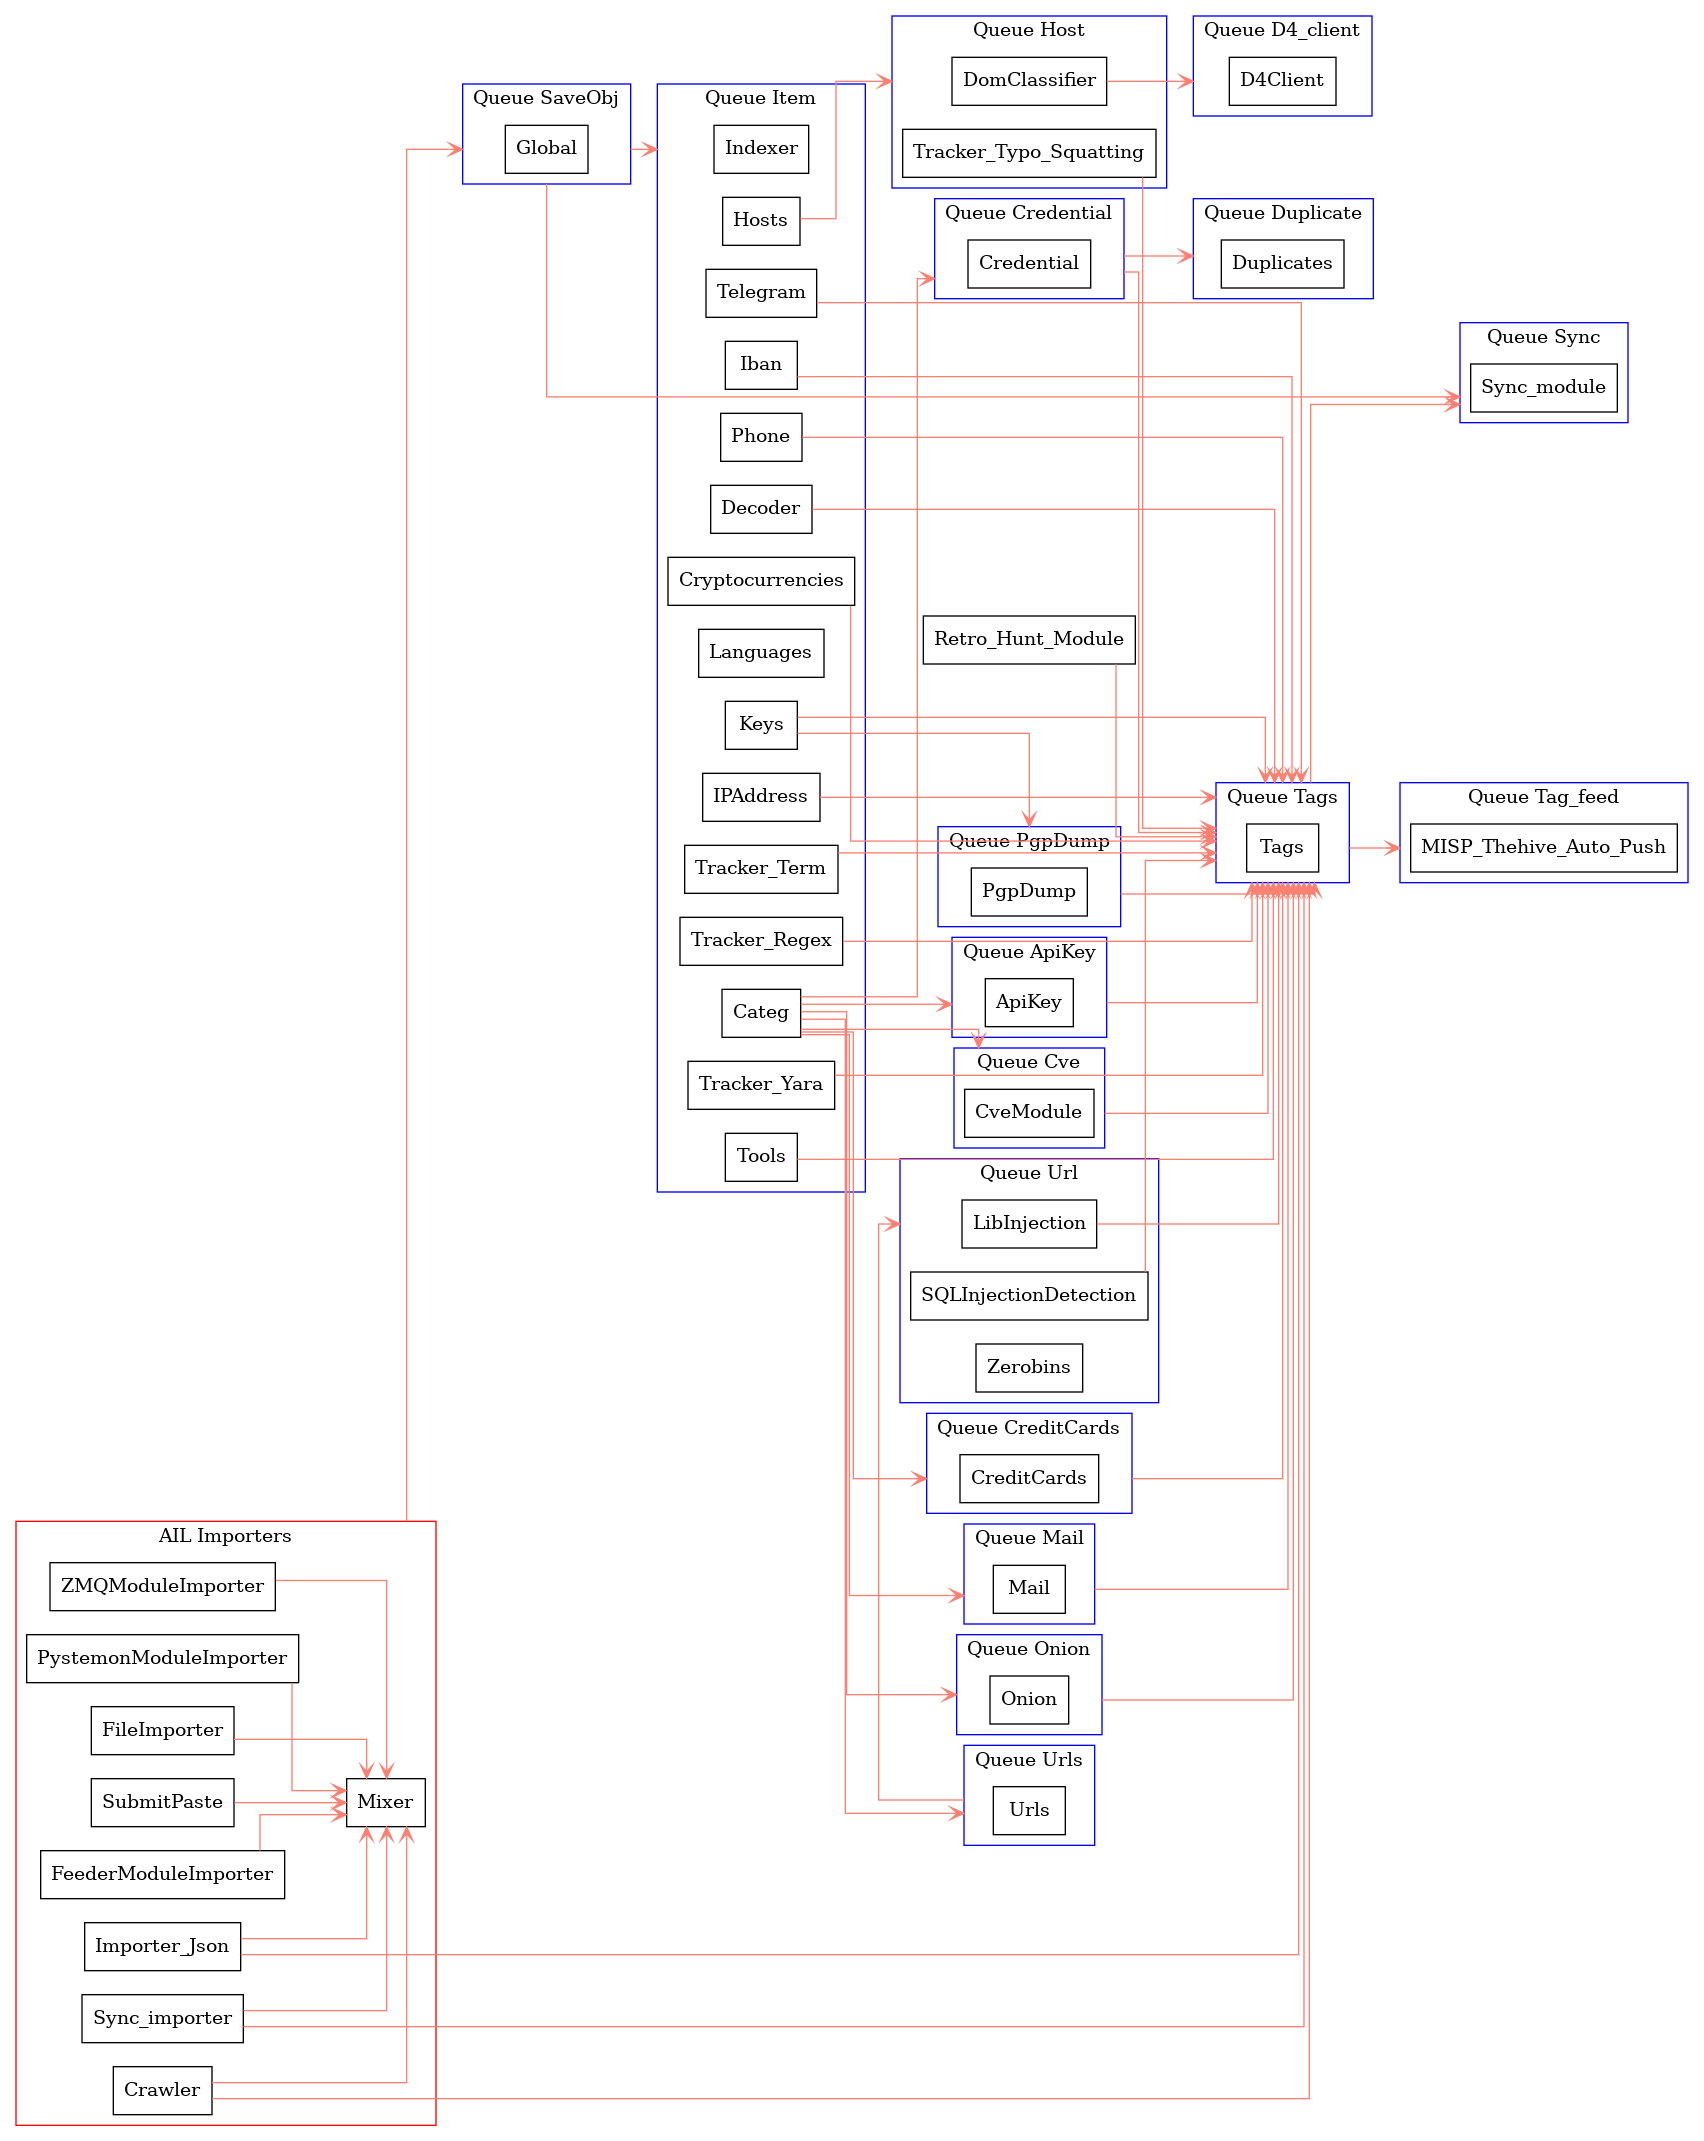
\includegraphics[scale=0.09]{images/ail_queues.png}}
\end{frame}

\begin{frame}
    \frametitle{AIL global architecture: Data streaming between module (Credential example)}
    \centerline{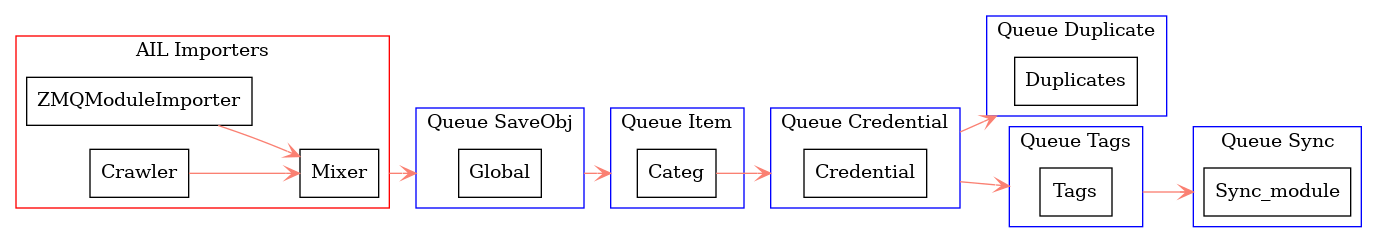
\includegraphics[scale=0.26]{images/ail_queues_credential.png}}
\end{frame}

\begin{frame}
    \frametitle{Message consuming}
    \begin{center}
    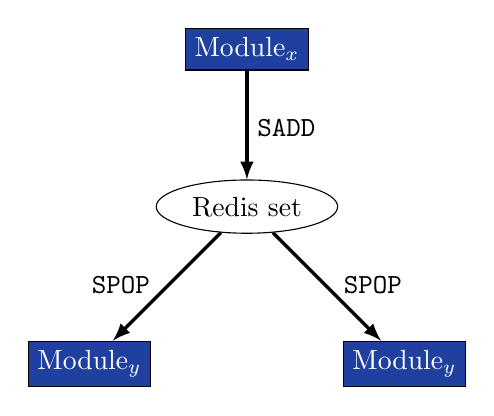
\begin{tikzpicture}[scale=1.0]
    %styles
    \tikzstyle{queue}=[ellipse,draw,align=center]
    \tikzstyle{module}=[rectangle,draw, align=center, fill={rgb:red,1;green,2;blue,5}]
    \tikzstyle{commu}=[->,>=latex,very thick]
    %nodes
    \node[module] (m0) at (0,2) {\color{white}Module$_x$};
    \node[queue] (rps1) at (0,0) {Redis set};
    \node[module] (m1) at (-2,-2) {\color{white}Module$_y$};
    \node[module] (m2) at (2,-2) {\color{white}Module$_y$};

    \node (t1) at (-1.6,-1) {\texttt{SPOP}};
    \node (t2) at (1.6,-1) {\texttt{SPOP}};
    \node (t3) at (0.5,1) {\texttt{SADD}};
    %arraws
    \draw[commu] (m0)--(rps1);
    \draw[commu] (rps1)--(m1);
    \draw[commu] (rps1)--(m2);

    \end{tikzpicture}


    \vskip 1em
    \begin{itemize}
        \item[] $\rightarrow$ No message lost nor double processing
        \item[] $\rightarrow$ Multiprocessing!
    \end{itemize}
    \end{center}
\end{frame}

%DEVELOPING NEW FEATURES
\section{Creating new features}
%Modules flow
\begin{frame}
    \frametitle{Developing new features: Plug-in a module in the system}
    \begin{enumerate}
        \item[] Choose where to put your module in the data flow:
    \end{enumerate}
    \begin{figure}
        \centerline{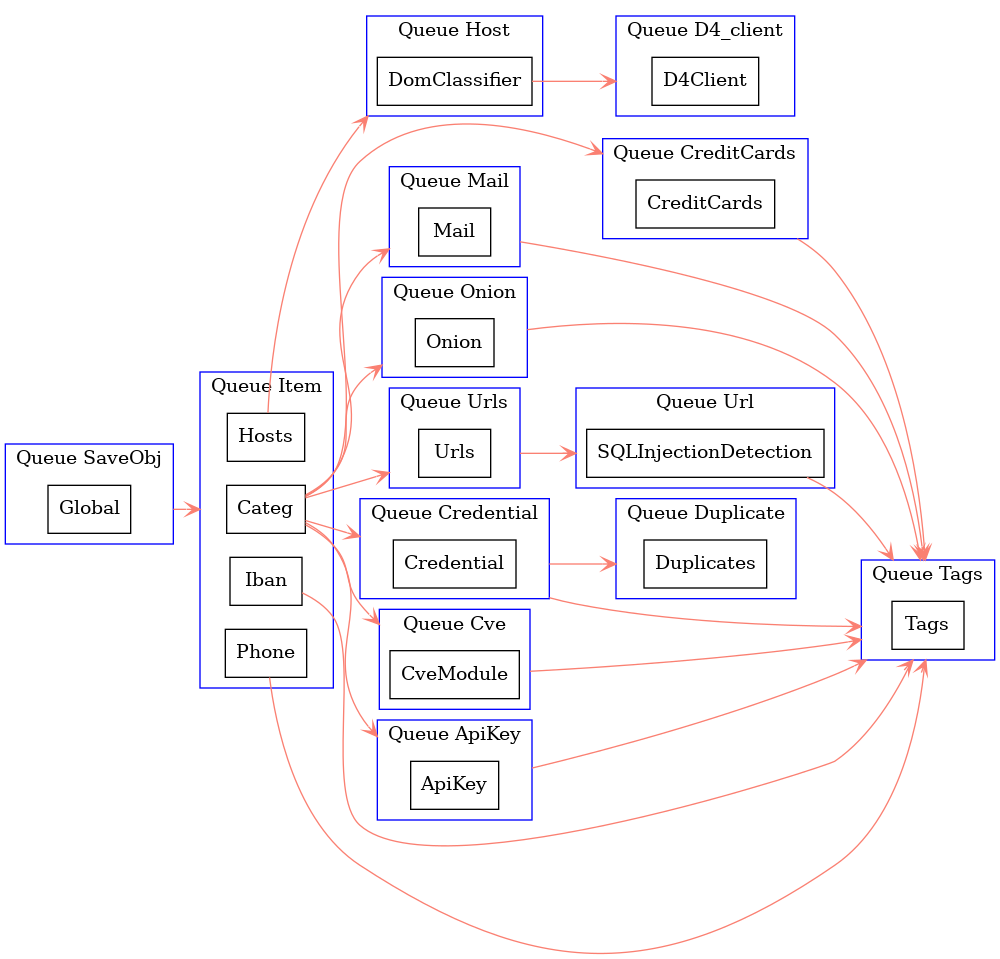
\includegraphics[scale=0.15]{images/ail_queues_simplified.png}}
    \end{figure}
    \vskip -1em
    \begin{enumerate}
        \item[] Then, modify \texttt{configs/modules.cfg} accordingly
    \end{enumerate}
\end{frame}


\lstset{style=code}
\lstset{basicstyle=\fontsize{6}{8}\ttfamily}
\begin{frame}[fragile]
    \frametitle{Writing your own modules - \texttt{/bin/modules/TemplateModule.py}}
    \begin{lstlisting}
from modules.abstract_module import AbstractModule

class NewModule(AbstractModule):

	def __init__(self):
        super().__init__()
		self.logger.info(f'Module {self.module_name} initialized')

	# Do something with the message from the queue
	def compute(self, message):
		# Process Message

# LAUNCH MODULE
if __name__ == '__main__':
    module = NewModule()
    module.run()

    \end{lstlisting}
\end{frame}

\lstset{style=code}
\lstset{basicstyle=\fontsize{6}{8}\ttfamily}
\begin{frame}[fragile]
    \frametitle{Writing your own Importer - \texttt{/bin/importer/}}
    \begin{lstlisting}
from importer.abstract_importer import AbstractImporter
from modules.abstract_module import AbstractModule

class MyNewImporter(AbstractImporter):

    def __init__(self):
        super().__init__()
        # super().__init__(queue=True)   # if it's an one-time run importer
        self.logger.info(f'Importer {self.name} initialized')

    def importer(self, my_var): # import function
        # Process my_var and get content to import
        content = GET_MY_CONTENT_TO_IMPORT
        # if content is not gzipped and/or not b64 encoded,
        # set gzipped and/or b64 to False
        message = self.create_message(item_id, content)
        return message
        # if it's an one-time run, otherwise create an AIL Module
        # self.add_message_to_queue(message)

class MyNewModuleImporter(AbstractModule):
    def __init__(self):
        super().__init__() # init module ...
        # init module ...
        self.importer = MyNewImporter()

    \end{lstlisting}
\end{frame}

\begin{frame}[fragile]
    \frametitle{Writing your own Importer - \texttt{/bin/importer/}}
    \begin{lstlisting}

    def get_message(self):
        return self.importer.importer()

    def compute(self, message):
        self.add_message_to_queue(message)

if __name__ == '__main__':
    module = MyNewModuleImporter()
    module.run()

    # if it's an one-time run:
    # importer = MyImporter()
    # importer.importer(my_var)

    \end{lstlisting}
\end{frame}

\section{Contribution rules}

\begin{frame}
\frametitle{How to contribute}
    \centerline{
\includegraphics[scale=0.33]{images/cat.png}}
\end{frame}

\begin{frame}
    \frametitle{Glimpse of contributed features}
    \begin{itemize}
        \item Docker
        \item Ansible
        \item Email alerting
        \item SQL injection detection
        \item Phone number detection
    \end{itemize}
\end{frame}


\begin{frame}
\frametitle{How to contribute}
%\o/
    \begin{itemize}
        \item Feel free to fork the code, play with it, make some patches or add additional analysis modules.
        \pause
        \item Feel free to make a pull request for your contribution
        \pause
        \item That's it!
    \end{itemize}
    \begin{figure}
        \includegraphics[scale=0.2]{images/dancing.png}
    \end{figure}
\end{frame}



\begin{frame}
   \frametitle{Final words}
   \begin{itemize}
        \item Building AIL helped us to find additional leaks which cannot be found using manual analysis and {\bf improve the time to detect duplicate/recycled leaks}.
            \vskip0.5cm
        \item[] $\rightarrow$ Therefore quicker response time to assist and/or inform proactively affected constituents.
   \end{itemize}
\end{frame}

\begin{frame}
    \frametitle{Implementation Steps in AIL project}
    \begin{itemize}
            \item {\bf Gradual changes} in AIL to add required functionalities to support the objectives.
            \item {\bf Time-memory trade-off} can be challenging to ensure a functional framework.
            \item Evaluation and integration of new modules in AIL based on time-memory comparisons.
            \item Semantic aspects are challenging due to the diverse data sources, unstructured data and languages seen.
    \end{itemize}
\end{frame}



\begin{frame}
    \frametitle{Ongoing Developments}
        \begin{itemize}
            \item Text Geolocation
            \item Improved MISP Export
            \item Bloom filter filtering - PSS
            \item Analysis of relationships and activity between chats, including message forwards, replies, timelines, etc.
            \item Improved indexing relying on Solr, Lucene or other components
            \item Integration with FlowIntel
        \end{itemize}
\end{frame}


\begin{frame}
    \frametitle{Private Search Set (PSS)}
    \begin{center}
        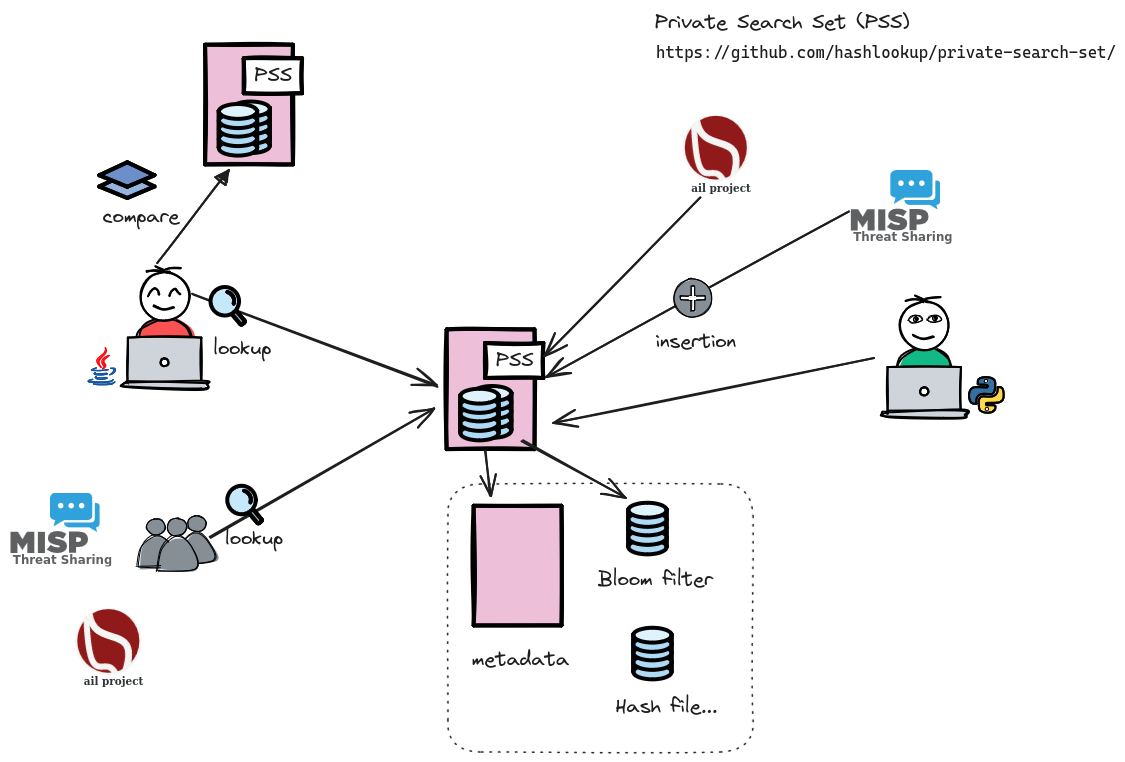
\includegraphics[scale=0.27]{images/pss-overview.png}
    \end{center}
\end{frame}


\section{Annexes}


%MANAGING THE SYSTEM
\subsection{Managing the framework}
\begin{frame}[fragile]
    \frametitle{Managing AIL: Old fashion way}
    \lstset{style=bash}
    \begin{tcblisting}{colback=black!85,coltext=green,listing only,
        title=Access the script screen, fonttitle=\bfseries}
screen -r Script
\end{tcblisting}
\begin{table}
        \caption{GNU screen shortcuts}
    \begin{tabular}{lr}
        \toprule
        Shortcut & Action \\
        \midrule
        C-a d & detach screen \\
        \midrule
        C-a c & Create new window \\
        \midrule
        C-a n & next window screen \\
        \midrule
        C-a p & previous window screen \\
        \bottomrule
    \end{tabular}
\end{table}
\end{frame}


\end{document}

